% Options for packages loaded elsewhere
\PassOptionsToPackage{unicode}{hyperref}
\PassOptionsToPackage{hyphens}{url}
\documentclass[
]{article}
\usepackage{xcolor}
\usepackage[margin=1in]{geometry}
\usepackage{amsmath,amssymb}
\setcounter{secnumdepth}{5}
\usepackage{iftex}
\ifPDFTeX
  \usepackage[T1]{fontenc}
  \usepackage[utf8]{inputenc}
  \usepackage{textcomp} % provide euro and other symbols
\else % if luatex or xetex
  \usepackage{unicode-math} % this also loads fontspec
  \defaultfontfeatures{Scale=MatchLowercase}
  \defaultfontfeatures[\rmfamily]{Ligatures=TeX,Scale=1}
\fi
\usepackage{lmodern}
\ifPDFTeX\else
  % xetex/luatex font selection
\fi
% Use upquote if available, for straight quotes in verbatim environments
\IfFileExists{upquote.sty}{\usepackage{upquote}}{}
\IfFileExists{microtype.sty}{% use microtype if available
  \usepackage[]{microtype}
  \UseMicrotypeSet[protrusion]{basicmath} % disable protrusion for tt fonts
}{}
\makeatletter
\@ifundefined{KOMAClassName}{% if non-KOMA class
  \IfFileExists{parskip.sty}{%
    \usepackage{parskip}
  }{% else
    \setlength{\parindent}{0pt}
    \setlength{\parskip}{6pt plus 2pt minus 1pt}}
}{% if KOMA class
  \KOMAoptions{parskip=half}}
\makeatother
\usepackage{color}
\usepackage{fancyvrb}
\newcommand{\VerbBar}{|}
\newcommand{\VERB}{\Verb[commandchars=\\\{\}]}
\DefineVerbatimEnvironment{Highlighting}{Verbatim}{commandchars=\\\{\}}
% Add ',fontsize=\small' for more characters per line
\usepackage{framed}
\definecolor{shadecolor}{RGB}{248,248,248}
\newenvironment{Shaded}{\begin{snugshade}}{\end{snugshade}}
\newcommand{\AlertTok}[1]{\textcolor[rgb]{0.94,0.16,0.16}{#1}}
\newcommand{\AnnotationTok}[1]{\textcolor[rgb]{0.56,0.35,0.01}{\textbf{\textit{#1}}}}
\newcommand{\AttributeTok}[1]{\textcolor[rgb]{0.13,0.29,0.53}{#1}}
\newcommand{\BaseNTok}[1]{\textcolor[rgb]{0.00,0.00,0.81}{#1}}
\newcommand{\BuiltInTok}[1]{#1}
\newcommand{\CharTok}[1]{\textcolor[rgb]{0.31,0.60,0.02}{#1}}
\newcommand{\CommentTok}[1]{\textcolor[rgb]{0.56,0.35,0.01}{\textit{#1}}}
\newcommand{\CommentVarTok}[1]{\textcolor[rgb]{0.56,0.35,0.01}{\textbf{\textit{#1}}}}
\newcommand{\ConstantTok}[1]{\textcolor[rgb]{0.56,0.35,0.01}{#1}}
\newcommand{\ControlFlowTok}[1]{\textcolor[rgb]{0.13,0.29,0.53}{\textbf{#1}}}
\newcommand{\DataTypeTok}[1]{\textcolor[rgb]{0.13,0.29,0.53}{#1}}
\newcommand{\DecValTok}[1]{\textcolor[rgb]{0.00,0.00,0.81}{#1}}
\newcommand{\DocumentationTok}[1]{\textcolor[rgb]{0.56,0.35,0.01}{\textbf{\textit{#1}}}}
\newcommand{\ErrorTok}[1]{\textcolor[rgb]{0.64,0.00,0.00}{\textbf{#1}}}
\newcommand{\ExtensionTok}[1]{#1}
\newcommand{\FloatTok}[1]{\textcolor[rgb]{0.00,0.00,0.81}{#1}}
\newcommand{\FunctionTok}[1]{\textcolor[rgb]{0.13,0.29,0.53}{\textbf{#1}}}
\newcommand{\ImportTok}[1]{#1}
\newcommand{\InformationTok}[1]{\textcolor[rgb]{0.56,0.35,0.01}{\textbf{\textit{#1}}}}
\newcommand{\KeywordTok}[1]{\textcolor[rgb]{0.13,0.29,0.53}{\textbf{#1}}}
\newcommand{\NormalTok}[1]{#1}
\newcommand{\OperatorTok}[1]{\textcolor[rgb]{0.81,0.36,0.00}{\textbf{#1}}}
\newcommand{\OtherTok}[1]{\textcolor[rgb]{0.56,0.35,0.01}{#1}}
\newcommand{\PreprocessorTok}[1]{\textcolor[rgb]{0.56,0.35,0.01}{\textit{#1}}}
\newcommand{\RegionMarkerTok}[1]{#1}
\newcommand{\SpecialCharTok}[1]{\textcolor[rgb]{0.81,0.36,0.00}{\textbf{#1}}}
\newcommand{\SpecialStringTok}[1]{\textcolor[rgb]{0.31,0.60,0.02}{#1}}
\newcommand{\StringTok}[1]{\textcolor[rgb]{0.31,0.60,0.02}{#1}}
\newcommand{\VariableTok}[1]{\textcolor[rgb]{0.00,0.00,0.00}{#1}}
\newcommand{\VerbatimStringTok}[1]{\textcolor[rgb]{0.31,0.60,0.02}{#1}}
\newcommand{\WarningTok}[1]{\textcolor[rgb]{0.56,0.35,0.01}{\textbf{\textit{#1}}}}
\usepackage{longtable,booktabs,array}
\newcounter{none} % for unnumbered tables
\usepackage{calc} % for calculating minipage widths
% Correct order of tables after \paragraph or \subparagraph
\usepackage{etoolbox}
\makeatletter
\patchcmd\longtable{\par}{\if@noskipsec\mbox{}\fi\par}{}{}
\makeatother
% Allow footnotes in longtable head/foot
\IfFileExists{footnotehyper.sty}{\usepackage{footnotehyper}}{\usepackage{footnote}}
\makesavenoteenv{longtable}
\usepackage{graphicx}
\makeatletter
\newsavebox\pandoc@box
\newcommand*\pandocbounded[1]{% scales image to fit in text height/width
  \sbox\pandoc@box{#1}%
  \Gscale@div\@tempa{\textheight}{\dimexpr\ht\pandoc@box+\dp\pandoc@box\relax}%
  \Gscale@div\@tempb{\linewidth}{\wd\pandoc@box}%
  \ifdim\@tempb\p@<\@tempa\p@\let\@tempa\@tempb\fi% select the smaller of both
  \ifdim\@tempa\p@<\p@\scalebox{\@tempa}{\usebox\pandoc@box}%
  \else\usebox{\pandoc@box}%
  \fi%
}
% Set default figure placement to htbp
\def\fps@figure{htbp}
\makeatother
\setlength{\emergencystretch}{3em} % prevent overfull lines
\providecommand{\tightlist}{%
  \setlength{\itemsep}{0pt}\setlength{\parskip}{0pt}}
\usepackage{booktabs}
\usepackage{longtable}
\usepackage{array}
\usepackage{multirow}
\usepackage{wrapfig}
\usepackage{float}
\usepackage{colortbl}
\usepackage{pdflscape}
\usepackage{tabu}
\usepackage{threeparttable}
\usepackage{threeparttablex}
\usepackage[normalem]{ulem}
\usepackage{makecell}
\usepackage{xcolor}
\usepackage{bookmark}
\IfFileExists{xurl.sty}{\usepackage{xurl}}{} % add URL line breaks if available
\urlstyle{same}
\hypersetup{
  pdftitle={Line-by-Line R Code Explanation --- Weibull Analysis Project},
  pdfauthor={{[}Author Name{]}},
  hidelinks,
  pdfcreator={LaTeX via pandoc}}

\title{Line-by-Line R Code Explanation --- Weibull Analysis Project}
\usepackage{etoolbox}
\makeatletter
\providecommand{\subtitle}[1]{% add subtitle to \maketitle
  \apptocmd{\@title}{\par {\large #1 \par}}{}{}
}
\makeatother
\subtitle{A Teaching Document for Students}
\author{{[}Author Name{]}}
\date{2026-04-23}

\begin{document}
\maketitle

{
\setcounter{tocdepth}{3}
\tableofcontents
}
\newpage

\section{Chapter 1 --- Data
Preparation}\label{chapter-1-data-preparation}

\subsection{1.1 Loading Multiple CSV
Files}\label{loading-multiple-csv-files}

\begin{Shaded}
\begin{Highlighting}[]
\NormalTok{df }\OtherTok{\textless{}{-}} \FunctionTok{list.files}\NormalTok{(}\StringTok{"data/"}\NormalTok{, }\AttributeTok{pattern =} \StringTok{"*.csv"}\NormalTok{, }\AttributeTok{full.names =} \ConstantTok{TRUE}\NormalTok{) }\SpecialCharTok{\%\textgreater{}\%}
  \FunctionTok{map\_dfr}\NormalTok{(read\_csv)}
\end{Highlighting}
\end{Shaded}

\textbf{What this does}: \texttt{list.files()} finds all CSV paths.
\texttt{map\_dfr(read\_csv)} applies \texttt{read\_csv} to each file and
row-binds (\texttt{\_dfr}) the results into one data frame.

\textbf{Why this matters}: Backblaze publishes one CSV per day. Manually
loading 92 files is impractical. \texttt{map\_dfr} automates this into a
single line.

\textbf{What breaks without it}: You would need a manual loop
(\texttt{for\ (f\ in\ files)\ \{\ ...\ rbind(...)\ \}}), achieving the
same result with more code and worse memory management.

\subsection{1.2 Collapsing to One Row Per
Drive}\label{collapsing-to-one-row-per-drive}

\begin{Shaded}
\begin{Highlighting}[]
\NormalTok{drives }\OtherTok{\textless{}{-}}\NormalTok{ df }\SpecialCharTok{\%\textgreater{}\%}
  \FunctionTok{group\_by}\NormalTok{(serial\_number) }\SpecialCharTok{\%\textgreater{}\%}
  \FunctionTok{summarise}\NormalTok{(}
    \AttributeTok{model         =} \FunctionTok{first}\NormalTok{(model),}
    \AttributeTok{first\_seen    =} \FunctionTok{min}\NormalTok{(date),}
    \AttributeTok{last\_seen     =} \FunctionTok{max}\NormalTok{(date),}
    \AttributeTok{failed        =} \FunctionTok{max}\NormalTok{(failure),}
    \AttributeTok{lifetime\_days =} \FunctionTok{as.numeric}\NormalTok{(last\_seen }\SpecialCharTok{{-}}\NormalTok{ first\_seen) }\SpecialCharTok{+} \DecValTok{1}
\NormalTok{  )}
\end{Highlighting}
\end{Shaded}

\textbf{What this does}: Groups all daily observations by
\texttt{serial\_number}, then computes one summary row per drive: the
model name, first/last observation dates, whether it ever failed, and
the observation window length.

\textbf{Why \texttt{max(failure)}}: If a drive has
\texttt{failure\ =\ 1} on any day, \texttt{max()} returns 1. All other
days are 0, so \texttt{max()} correctly identifies ever-failed drives.

\textbf{Why \texttt{+1}}:
\texttt{as.numeric(last\_seen\ -\ first\_seen)} for a drive seen only on
July 1st gives 0 days. But it existed for 1 day. The \texttt{+1} ensures
\texttt{lifetime\_days\ \textgreater{}=\ 1}, preventing
\texttt{log(0)\ =\ -Inf} in all Weibull linearizations.

\textbf{\texttt{failed\ =\ 0} (right-censoring)}: The drive survived at
least this long. Its exact failure time is unknown. Ignoring these
drives means we only observe short-lived drives, biasing all estimates
downward.

\subsection{1.3 Removing Invalid
Lifetimes}\label{removing-invalid-lifetimes}

\begin{Shaded}
\begin{Highlighting}[]
\NormalTok{drives }\OtherTok{\textless{}{-}}\NormalTok{ drives }\SpecialCharTok{\%\textgreater{}\%} \FunctionTok{filter}\NormalTok{(lifetime\_days }\SpecialCharTok{\textgreater{}} \DecValTok{0}\NormalTok{)}
\end{Highlighting}
\end{Shaded}

\textbf{What this does}: Removes drives with
\texttt{lifetime\_days\ \textless{}=\ 0} (data artifacts from date
parsing errors).

\textbf{What breaks without it}: \texttt{log(0)\ =\ -Inf} in Weibull
probability paper. \texttt{0\^{}k\ =\ 0} causes \texttt{log(0)} in MLE.
Every method fails.

\newpage

\section{Chapter 2 --- Estimation
Methods}\label{chapter-2-estimation-methods}

\subsection{Toy Dataset for Worked
Examples}\label{toy-dataset-for-worked-examples}

All methods are demonstrated on the same toy dataset:

\begin{Shaded}
\begin{Highlighting}[]
\NormalTok{toy\_t }\OtherTok{\textless{}{-}} \FunctionTok{c}\NormalTok{(}\DecValTok{120}\NormalTok{, }\DecValTok{340}\NormalTok{, }\DecValTok{580}\NormalTok{, }\DecValTok{720}\NormalTok{, }\DecValTok{950}\NormalTok{, }\DecValTok{1100}\NormalTok{, }\DecValTok{1380}\NormalTok{, }\DecValTok{1650}\NormalTok{, }\DecValTok{2100}\NormalTok{, }\DecValTok{2800}\NormalTok{)}
\NormalTok{toy\_n }\OtherTok{\textless{}{-}} \FunctionTok{length}\NormalTok{(toy\_t)}
\FunctionTok{cat}\NormalTok{(}\StringTok{"Toy data: n ="}\NormalTok{, toy\_n, }\StringTok{"failure times}\SpecialCharTok{\textbackslash{}n}\StringTok{"}\NormalTok{)}
\end{Highlighting}
\end{Shaded}

\begin{verbatim}
## Toy data: n = 10 failure times
\end{verbatim}

\begin{Shaded}
\begin{Highlighting}[]
\FunctionTok{cat}\NormalTok{(}\StringTok{"Mean ="}\NormalTok{, }\FunctionTok{mean}\NormalTok{(toy\_t), }\StringTok{"| SD ="}\NormalTok{, }\FunctionTok{sd}\NormalTok{(toy\_t), }\StringTok{"| Min ="}\NormalTok{, }\FunctionTok{min}\NormalTok{(toy\_t), }\StringTok{"| Max ="}\NormalTok{, }\FunctionTok{max}\NormalTok{(toy\_t))}
\end{Highlighting}
\end{Shaded}

\begin{verbatim}
## Mean = 1174 | SD = 829.42 | Min = 120 | Max = 2800
\end{verbatim}

\subsection{2.1 OLS (also known as MRR)}\label{ols-also-known-as-mrr}

\subsubsection{2.1.1 Mathematical
Foundation}\label{mathematical-foundation}

The Weibull CDF is:
\[F(t) = 1 - \exp\left(-\left(\frac{t}{\lambda}\right)^k\right)\]

Taking logarithms twice:
\[\ln(1-F) = -\left(\frac{t}{\lambda}\right)^k\]
\[\ln(-\ln(1-F)) = k \cdot \ln(t) - k \cdot \ln(\lambda)\]

This is a straight line \(Y = k \cdot X + b\) where: -
\(Y_i = \ln(-\ln(1-F_i))\) - \(X_i = \ln(t_i)\) - Slope \(= k\) -
Intercept \(b = -k \cdot \ln(\lambda)\), so \(\lambda = \exp(-b/k)\)

\textbf{Benard's formula} for median ranks:
\[\hat{F}_i = \frac{i - 0.3}{n + 0.4}\]

Why not \(i/n\): the last point gives \(F_n = 1\), then
\(\ln(-\ln(0)) = -\infty\). Benard's formula approximates the median of
the \(\text{Beta}(i, n-i+1)\) distribution.

\subsubsection{2.1.2 R Code Line by Line}\label{r-code-line-by-line}

\begin{Shaded}
\begin{Highlighting}[]
\CommentTok{\# Step 1: Sort failure times ascending}
\NormalTok{t\_sorted }\OtherTok{\textless{}{-}} \FunctionTok{sort}\NormalTok{(toy\_t)}

\CommentTok{\# Step 2: Compute median ranks (Benard\textquotesingle{}s formula)}
\NormalTok{n }\OtherTok{\textless{}{-}} \FunctionTok{length}\NormalTok{(t\_sorted)}
\NormalTok{i }\OtherTok{\textless{}{-}} \DecValTok{1}\SpecialCharTok{:}\NormalTok{n}
\NormalTok{F\_i }\OtherTok{\textless{}{-}}\NormalTok{ (i }\SpecialCharTok{{-}} \FloatTok{0.3}\NormalTok{) }\SpecialCharTok{/}\NormalTok{ (n }\SpecialCharTok{+} \FloatTok{0.4}\NormalTok{)}

\FunctionTok{cat}\NormalTok{(}\StringTok{"Rank  Time   F\_i (Benard)}\SpecialCharTok{\textbackslash{}n}\StringTok{"}\NormalTok{)}
\end{Highlighting}
\end{Shaded}

\begin{verbatim}
## Rank  Time   F_i (Benard)
\end{verbatim}

\begin{Shaded}
\begin{Highlighting}[]
\ControlFlowTok{for}\NormalTok{ (j }\ControlFlowTok{in} \DecValTok{1}\SpecialCharTok{:}\NormalTok{n) }\FunctionTok{cat}\NormalTok{(}\FunctionTok{sprintf}\NormalTok{(}\StringTok{"  \%2d  \%5d   \%.4f}\SpecialCharTok{\textbackslash{}n}\StringTok{"}\NormalTok{, j, t\_sorted[j], F\_i[j]))}
\end{Highlighting}
\end{Shaded}

\begin{verbatim}
##    1    120   0.0673
##    2    340   0.1635
##    3    580   0.2596
##    4    720   0.3558
##    5    950   0.4519
##    6   1100   0.5481
##    7   1380   0.6442
##    8   1650   0.7404
##    9   2100   0.8365
##   10   2800   0.9327
\end{verbatim}

\begin{Shaded}
\begin{Highlighting}[]
\CommentTok{\# Step 3: Weibull linearization}
\NormalTok{Y }\OtherTok{\textless{}{-}} \FunctionTok{log}\NormalTok{(}\SpecialCharTok{{-}}\FunctionTok{log}\NormalTok{(}\DecValTok{1} \SpecialCharTok{{-}}\NormalTok{ F\_i))   }\CommentTok{\# Double{-}log transform}
\NormalTok{X }\OtherTok{\textless{}{-}} \FunctionTok{log}\NormalTok{(t\_sorted)         }\CommentTok{\# Log of failure times}

\CommentTok{\# Step 4: OLS regression — NO weights}
\NormalTok{fit\_ols }\OtherTok{\textless{}{-}} \FunctionTok{lm}\NormalTok{(Y }\SpecialCharTok{\textasciitilde{}}\NormalTok{ X)}
\NormalTok{k\_ols }\OtherTok{\textless{}{-}} \FunctionTok{unname}\NormalTok{(}\FunctionTok{coef}\NormalTok{(fit\_ols)[}\DecValTok{2}\NormalTok{])           }\CommentTok{\# slope = k}
\NormalTok{lam\_ols }\OtherTok{\textless{}{-}} \FunctionTok{exp}\NormalTok{(}\SpecialCharTok{{-}}\FunctionTok{unname}\NormalTok{(}\FunctionTok{coef}\NormalTok{(fit\_ols)[}\DecValTok{1}\NormalTok{]) }\SpecialCharTok{/}\NormalTok{ k\_ols)  }\CommentTok{\# lambda}

\FunctionTok{cat}\NormalTok{(}\StringTok{"OLS results: k ="}\NormalTok{, }\FunctionTok{round}\NormalTok{(k\_ols, }\DecValTok{4}\NormalTok{), }\StringTok{", lambda ="}\NormalTok{, }\FunctionTok{round}\NormalTok{(lam\_ols, }\DecValTok{2}\NormalTok{))}
\end{Highlighting}
\end{Shaded}

\begin{verbatim}
## OLS results: k = 1.1881 , lambda = 1345.69
\end{verbatim}

\textbf{Why OLS is biased}: The \(i\)-th order statistic from \(N\)
uniform draws has variance
\(\text{Var}(F_i) = \frac{i(N-i+1)}{(N+1)^2(N+2)}\). This is large at
the tails (\(i=1\) or \(i=N\)), small in the middle. OLS treats every
residual equally, so tail points with high noise drag the regression
line.

\subsubsection{2.1.3 Worked Numerical
Example}\label{worked-numerical-example}

\begin{Shaded}
\begin{Highlighting}[]
\FunctionTok{cat}\NormalTok{(}\StringTok{"X (log t):"}\NormalTok{, }\FunctionTok{round}\NormalTok{(X, }\DecValTok{3}\NormalTok{), }\StringTok{"}\SpecialCharTok{\textbackslash{}n}\StringTok{"}\NormalTok{)}
\end{Highlighting}
\end{Shaded}

\begin{verbatim}
## X (log t): 4.787 5.829 6.363 6.579 6.856 7.003 7.23 7.409 7.65 7.937
\end{verbatim}

\begin{Shaded}
\begin{Highlighting}[]
\FunctionTok{cat}\NormalTok{(}\StringTok{"Y (log({-}log(1{-}F))):"}\NormalTok{, }\FunctionTok{round}\NormalTok{(Y, }\DecValTok{3}\NormalTok{), }\StringTok{"}\SpecialCharTok{\textbackslash{}n}\StringTok{"}\NormalTok{)}
\end{Highlighting}
\end{Shaded}

\begin{verbatim}
## Y (log(-log(1-F))): -2.664 -1.723 -1.202 -0.822 -0.509 -0.23 0.033 0.299 0.594 0.993
\end{verbatim}

\begin{Shaded}
\begin{Highlighting}[]
\FunctionTok{cat}\NormalTok{(}\StringTok{"}\SpecialCharTok{\textbackslash{}n}\StringTok{Regression: Y = "}\NormalTok{, }\FunctionTok{round}\NormalTok{(}\FunctionTok{coef}\NormalTok{(fit\_ols)[}\DecValTok{2}\NormalTok{], }\DecValTok{4}\NormalTok{), }\StringTok{"* X + ("}\NormalTok{,}
    \FunctionTok{round}\NormalTok{(}\FunctionTok{coef}\NormalTok{(fit\_ols)[}\DecValTok{1}\NormalTok{], }\DecValTok{4}\NormalTok{), }\StringTok{")}\SpecialCharTok{\textbackslash{}n}\StringTok{"}\NormalTok{)}
\end{Highlighting}
\end{Shaded}

\begin{verbatim}
## 
## Regression: Y =  1.1881 * X + ( -8.5599 )
\end{verbatim}

\begin{Shaded}
\begin{Highlighting}[]
\FunctionTok{cat}\NormalTok{(}\StringTok{"k ="}\NormalTok{, }\FunctionTok{round}\NormalTok{(k\_ols, }\DecValTok{4}\NormalTok{), }\StringTok{"}\SpecialCharTok{\textbackslash{}n}\StringTok{"}\NormalTok{)}
\end{Highlighting}
\end{Shaded}

\begin{verbatim}
## k = 1.1881
\end{verbatim}

\begin{Shaded}
\begin{Highlighting}[]
\FunctionTok{cat}\NormalTok{(}\StringTok{"lambda = exp({-}"}\NormalTok{, }\FunctionTok{round}\NormalTok{(}\FunctionTok{coef}\NormalTok{(fit\_ols)[}\DecValTok{1}\NormalTok{], }\DecValTok{4}\NormalTok{), }\StringTok{"/"}\NormalTok{, }\FunctionTok{round}\NormalTok{(k\_ols, }\DecValTok{4}\NormalTok{),}
    \StringTok{") ="}\NormalTok{, }\FunctionTok{round}\NormalTok{(lam\_ols, }\DecValTok{2}\NormalTok{), }\StringTok{"}\SpecialCharTok{\textbackslash{}n}\StringTok{"}\NormalTok{)}
\end{Highlighting}
\end{Shaded}

\begin{verbatim}
## lambda = exp(- -8.5599 / 1.1881 ) = 1345.69
\end{verbatim}

\subsection{2.2 WLS (Weighted Least Squares --- Bergman
Weights)}\label{wls-weighted-least-squares-bergman-weights}

\subsubsection{2.2.1 Mathematical
Foundation}\label{mathematical-foundation-1}

\textbf{4-Step Bergman weight derivation}:

\begin{enumerate}
\def\labelenumi{\arabic{enumi}.}
\tightlist
\item
  \(\text{Var}(F_i) = \frac{i(N-i+1)}{(N+1)^2(N+2)}\) (Beta distribution
  variance)
\item
  \(g'(F_i) = \frac{1}{(1-F_i)(-\ln(1-F_i))}\) (chain rule on
  \(Y = g(F)\))
\item
  \(\text{Var}(Y_i) \approx [g'(F_i)]^2 \cdot \text{Var}(F_i)\) (delta
  method)
\item
  \(w_i = 1/\text{Var}(Y_i)\) (WLS weight)
\end{enumerate}

Combined:
\[w_i = \frac{[(1-F_i)(-\ln(1-F_i))]^2 \cdot (N+1)^2(N+2)}{i(N-i+1)}\]

\textbf{Weight peak at \(F \approx 0.632\)}: Maximize
\(f(s) = -s \ln(s)\) where \(s = 1-F\):
\(f'(s) = -\ln(s) - 1 = 0 \Rightarrow s = e^{-1} \Rightarrow F = 1 - e^{-1} \approx 0.632\).
This is \(t = \lambda\) (the Weibull characteristic life).

\subsubsection{2.2.2 R Code Line by Line}\label{r-code-line-by-line-1}

\begin{Shaded}
\begin{Highlighting}[]
\CommentTok{\# Bergman weights}
\NormalTok{wi }\OtherTok{\textless{}{-}}\NormalTok{ ((}\DecValTok{1} \SpecialCharTok{{-}}\NormalTok{ F\_i) }\SpecialCharTok{*}\NormalTok{ (}\SpecialCharTok{{-}}\FunctionTok{log}\NormalTok{(}\DecValTok{1} \SpecialCharTok{{-}}\NormalTok{ F\_i)))}\SpecialCharTok{\^{}}\DecValTok{2} \SpecialCharTok{*}\NormalTok{ (n }\SpecialCharTok{+} \DecValTok{1}\NormalTok{)}\SpecialCharTok{\^{}}\DecValTok{2} \SpecialCharTok{*}\NormalTok{ (n }\SpecialCharTok{+} \DecValTok{2}\NormalTok{) }\SpecialCharTok{/}\NormalTok{ (i }\SpecialCharTok{*}\NormalTok{ (n }\SpecialCharTok{{-}}\NormalTok{ i }\SpecialCharTok{+} \DecValTok{1}\NormalTok{))}

\FunctionTok{cat}\NormalTok{(}\StringTok{"Rank  F\_i      Weight (normalized)}\SpecialCharTok{\textbackslash{}n}\StringTok{"}\NormalTok{)}
\end{Highlighting}
\end{Shaded}

\begin{verbatim}
## Rank  F_i      Weight (normalized)
\end{verbatim}

\begin{Shaded}
\begin{Highlighting}[]
\ControlFlowTok{for}\NormalTok{ (j }\ControlFlowTok{in} \DecValTok{1}\SpecialCharTok{:}\NormalTok{n) }\FunctionTok{cat}\NormalTok{(}\FunctionTok{sprintf}\NormalTok{(}\StringTok{"  \%2d   \%.4f   \%.4f}\SpecialCharTok{\textbackslash{}n}\StringTok{"}\NormalTok{, j, F\_i[j], wi[j]}\SpecialCharTok{/}\FunctionTok{max}\NormalTok{(wi)))}
\end{Highlighting}
\end{Shaded}

\begin{verbatim}
##    1   0.0673   0.0827
##    2   0.1635   0.2425
##    3   0.2596   0.4041
##    4   0.3558   0.5611
##    5   0.4519   0.7089
##    6   0.5481   0.8409
##    7   0.6442   0.9453
##    8   0.7404   1.0000
##    9   0.8365   0.9534
##   10   0.9327   0.6459
\end{verbatim}

\begin{Shaded}
\begin{Highlighting}[]
\CommentTok{\# WLS regression}
\NormalTok{fit\_wls }\OtherTok{\textless{}{-}} \FunctionTok{lm}\NormalTok{(Y }\SpecialCharTok{\textasciitilde{}}\NormalTok{ X, }\AttributeTok{weights =}\NormalTok{ wi)}
\NormalTok{k\_wls }\OtherTok{\textless{}{-}} \FunctionTok{unname}\NormalTok{(}\FunctionTok{coef}\NormalTok{(fit\_wls)[}\DecValTok{2}\NormalTok{])}
\NormalTok{lam\_wls }\OtherTok{\textless{}{-}} \FunctionTok{exp}\NormalTok{(}\SpecialCharTok{{-}}\FunctionTok{unname}\NormalTok{(}\FunctionTok{coef}\NormalTok{(fit\_wls)[}\DecValTok{1}\NormalTok{]) }\SpecialCharTok{/}\NormalTok{ k\_wls)}
\FunctionTok{cat}\NormalTok{(}\StringTok{"}\SpecialCharTok{\textbackslash{}n}\StringTok{WLS results: k ="}\NormalTok{, }\FunctionTok{round}\NormalTok{(k\_wls, }\DecValTok{4}\NormalTok{), }\StringTok{", lambda ="}\NormalTok{, }\FunctionTok{round}\NormalTok{(lam\_wls, }\DecValTok{2}\NormalTok{))}
\end{Highlighting}
\end{Shaded}

\begin{verbatim}
## 
## WLS results: k = 1.2852 , lambda = 1335.7
\end{verbatim}

\subsubsection{WLS Weight Visualization}\label{wls-weight-visualization}

\begin{Shaded}
\begin{Highlighting}[]
\CommentTok{\# Hypothetical n=20 to show weight pattern clearly}
\NormalTok{n\_hyp }\OtherTok{\textless{}{-}} \DecValTok{20}
\NormalTok{i\_hyp }\OtherTok{\textless{}{-}} \DecValTok{1}\SpecialCharTok{:}\NormalTok{n\_hyp}
\NormalTok{F\_hyp }\OtherTok{\textless{}{-}}\NormalTok{ (i\_hyp }\SpecialCharTok{{-}} \FloatTok{0.3}\NormalTok{) }\SpecialCharTok{/}\NormalTok{ (n\_hyp }\SpecialCharTok{+} \FloatTok{0.4}\NormalTok{)}
\NormalTok{wi\_hyp }\OtherTok{\textless{}{-}}\NormalTok{ ((}\DecValTok{1} \SpecialCharTok{{-}}\NormalTok{ F\_hyp) }\SpecialCharTok{*}\NormalTok{ (}\SpecialCharTok{{-}}\FunctionTok{log}\NormalTok{(}\DecValTok{1} \SpecialCharTok{{-}}\NormalTok{ F\_hyp)))}\SpecialCharTok{\^{}}\DecValTok{2} \SpecialCharTok{*}\NormalTok{ (n\_hyp }\SpecialCharTok{+} \DecValTok{1}\NormalTok{)}\SpecialCharTok{\^{}}\DecValTok{2} \SpecialCharTok{*}\NormalTok{ (n\_hyp }\SpecialCharTok{+} \DecValTok{2}\NormalTok{) }\SpecialCharTok{/}
\NormalTok{  (i\_hyp }\SpecialCharTok{*}\NormalTok{ (n\_hyp }\SpecialCharTok{{-}}\NormalTok{ i\_hyp }\SpecialCharTok{+} \DecValTok{1}\NormalTok{))}
\NormalTok{wi\_norm }\OtherTok{\textless{}{-}}\NormalTok{ wi\_hyp }\SpecialCharTok{/} \FunctionTok{max}\NormalTok{(wi\_hyp)}

\CommentTok{\# Find peak position}
\NormalTok{peak\_idx }\OtherTok{\textless{}{-}} \FunctionTok{which.max}\NormalTok{(wi\_norm)}
\NormalTok{peak\_F }\OtherTok{\textless{}{-}}\NormalTok{ F\_hyp[peak\_idx]}

\FunctionTok{ggplot}\NormalTok{(}\FunctionTok{tibble}\NormalTok{(}\AttributeTok{rank =}\NormalTok{ i\_hyp, }\AttributeTok{weight =}\NormalTok{ wi\_norm, }\AttributeTok{F\_val =}\NormalTok{ F\_hyp),}
       \FunctionTok{aes}\NormalTok{(}\AttributeTok{x =}\NormalTok{ rank, }\AttributeTok{y =}\NormalTok{ weight)) }\SpecialCharTok{+}
  \FunctionTok{geom\_line}\NormalTok{(}\AttributeTok{color =} \StringTok{"\#377EB8"}\NormalTok{, }\AttributeTok{linewidth =} \DecValTok{1}\NormalTok{) }\SpecialCharTok{+}
  \FunctionTok{geom\_point}\NormalTok{(}\AttributeTok{color =} \StringTok{"\#377EB8"}\NormalTok{, }\AttributeTok{size =} \DecValTok{2}\NormalTok{) }\SpecialCharTok{+}
  \FunctionTok{geom\_vline}\NormalTok{(}\AttributeTok{xintercept =}\NormalTok{ peak\_idx, }\AttributeTok{linetype =} \StringTok{"dashed"}\NormalTok{, }\AttributeTok{color =} \StringTok{"red"}\NormalTok{) }\SpecialCharTok{+}
  \FunctionTok{annotate}\NormalTok{(}\StringTok{"text"}\NormalTok{, }\AttributeTok{x =}\NormalTok{ peak\_idx }\SpecialCharTok{+} \DecValTok{1}\NormalTok{, }\AttributeTok{y =} \FloatTok{0.95}\NormalTok{,}
           \AttributeTok{label =} \FunctionTok{paste0}\NormalTok{(}\StringTok{"Peak at F ≈ "}\NormalTok{, }\FunctionTok{round}\NormalTok{(peak\_F, }\DecValTok{3}\NormalTok{), }\StringTok{" ≈ 0.632"}\NormalTok{),}
           \AttributeTok{hjust =} \DecValTok{0}\NormalTok{, }\AttributeTok{size =} \FloatTok{3.5}\NormalTok{, }\AttributeTok{color =} \StringTok{"red"}\NormalTok{) }\SpecialCharTok{+}
  \FunctionTok{annotate}\NormalTok{(}\StringTok{"text"}\NormalTok{, }\AttributeTok{x =} \DecValTok{2}\NormalTok{, }\AttributeTok{y =} \FloatTok{0.15}\NormalTok{, }\AttributeTok{label =} \StringTok{"Tail ranks:}\SpecialCharTok{\textbackslash{}n}\StringTok{near{-}zero weight"}\NormalTok{,}
           \AttributeTok{size =} \DecValTok{3}\NormalTok{, }\AttributeTok{color =} \StringTok{"grey40"}\NormalTok{) }\SpecialCharTok{+}
  \FunctionTok{annotate}\NormalTok{(}\StringTok{"text"}\NormalTok{, }\AttributeTok{x =} \DecValTok{19}\NormalTok{, }\AttributeTok{y =} \FloatTok{0.15}\NormalTok{, }\AttributeTok{label =} \StringTok{"Tail ranks:}\SpecialCharTok{\textbackslash{}n}\StringTok{near{-}zero weight"}\NormalTok{,}
           \AttributeTok{size =} \DecValTok{3}\NormalTok{, }\AttributeTok{color =} \StringTok{"grey40"}\NormalTok{) }\SpecialCharTok{+}
  \FunctionTok{labs}\NormalTok{(}\AttributeTok{title =} \StringTok{"Bergman WLS Weights Across Ranks (n=20)"}\NormalTok{,}
       \AttributeTok{subtitle =} \StringTok{"OLS treats all ranks equally (horizontal line at weight=1)"}\NormalTok{,}
       \AttributeTok{x =} \StringTok{"Rank i"}\NormalTok{, }\AttributeTok{y =} \StringTok{"Normalized Weight"}\NormalTok{) }\SpecialCharTok{+}
  \FunctionTok{theme\_bw}\NormalTok{()}
\end{Highlighting}
\end{Shaded}

\begin{figure}[H]

{\centering 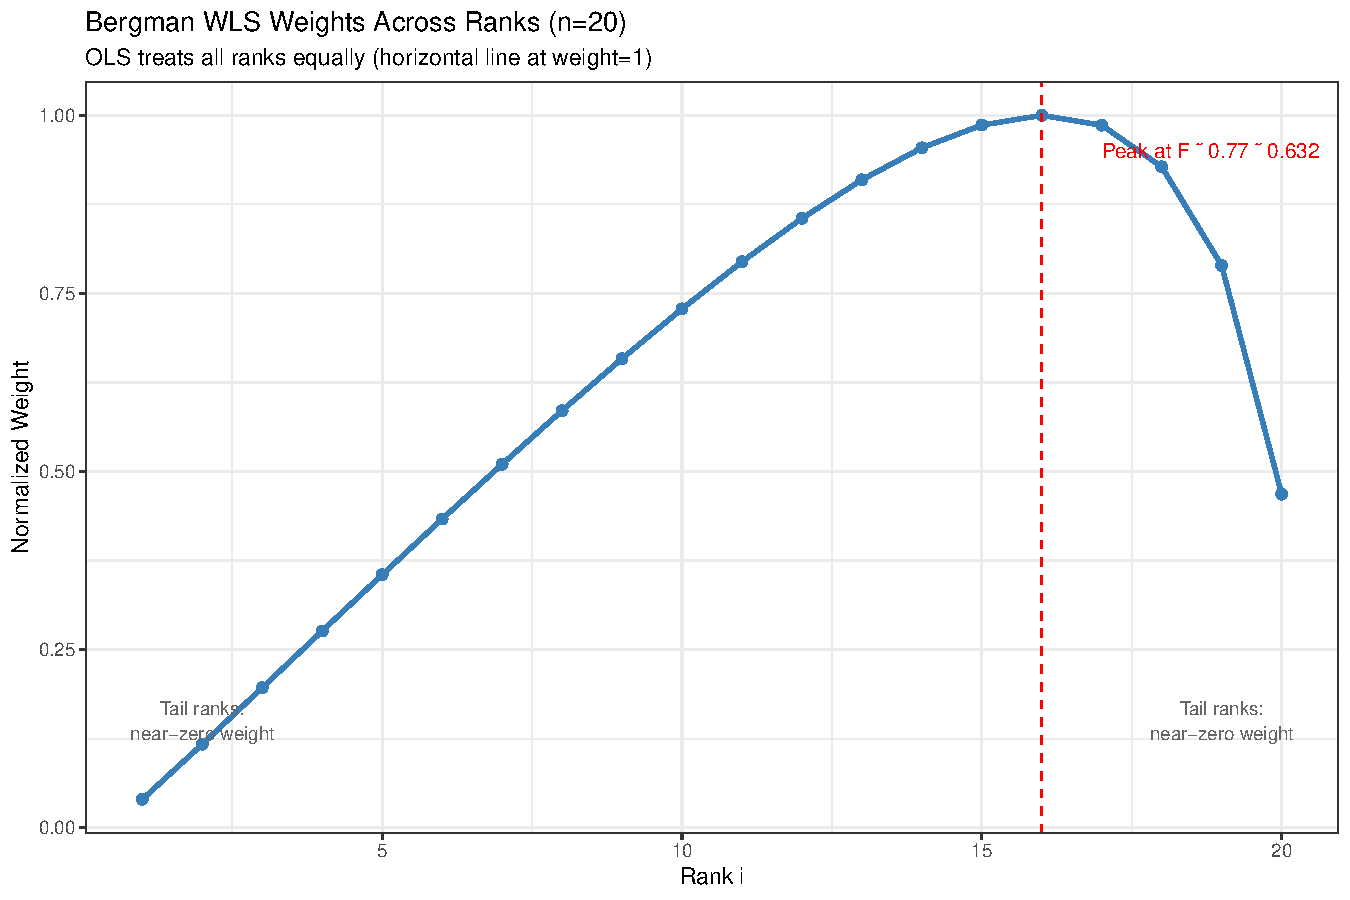
\includegraphics{CODE_EXPLAINED_files/figure-latex/wls-weight-plot-1} 

}

\caption{Bergman weights across ranks for n=20}\label{fig:wls-weight-plot}
\end{figure}

\textbf{WLS vs L-Moments on outliers}: WLS handles predictable
rank-position noise (Beta variance). A genuinely anomalous data point at
a middle rank gets HIGH WLS weight --- bad. L-Moments handles true
outliers via linear combinations.

\textbf{WLS can outrank MLE}: If the true distribution is only
approximately Weibull, MLE's commitment to the exact functional form is
a liability. WLS fits the empirical CDF more loosely.

\subsection{2.3 MOM (Method of Moments)}\label{mom-method-of-moments}

\subsubsection{2.3.1 Mathematical
Foundation}\label{mathematical-foundation-2}

Weibull moments:
\[E[T] = \lambda \Gamma\left(1 + \frac{1}{k}\right), \quad \text{Var}(T) = \lambda^2\left[\Gamma\left(1+\frac{2}{k}\right) - \Gamma\left(1+\frac{1}{k}\right)^2\right]\]

\textbf{Squared coefficient of variation}:
\[CV^2 = \frac{\Gamma(1+2/k)}{\Gamma(1+1/k)^2} - 1\]

\textbf{UNIVERSAL PATTERN}: \(\lambda\) is a pure scale parameter. Any
dimensionless ratio of moments has \(\lambda\) cancel exactly. \(CV^2\),
\(\tau_2\) (L-Moments), and \(EPF\) all depend only on \(k\). This is
referenced by Methods 4 and 5.

\subsubsection{2.3.2 R Code Line by Line}\label{r-code-line-by-line-2}

\begin{Shaded}
\begin{Highlighting}[]
\NormalTok{mu }\OtherTok{\textless{}{-}} \FunctionTok{mean}\NormalTok{(toy\_t)}
\NormalTok{sigma2 }\OtherTok{\textless{}{-}} \FunctionTok{var}\NormalTok{(toy\_t)}
\NormalTok{CV2 }\OtherTok{\textless{}{-}}\NormalTok{ sigma2 }\SpecialCharTok{/}\NormalTok{ mu}\SpecialCharTok{\^{}}\DecValTok{2}
\FunctionTok{cat}\NormalTok{(}\StringTok{"mu ="}\NormalTok{, }\FunctionTok{round}\NormalTok{(mu, }\DecValTok{2}\NormalTok{), }\StringTok{"| var ="}\NormalTok{, }\FunctionTok{round}\NormalTok{(sigma2, }\DecValTok{2}\NormalTok{), }\StringTok{"| CV² ="}\NormalTok{, }\FunctionTok{round}\NormalTok{(CV2, }\DecValTok{4}\NormalTok{), }\StringTok{"}\SpecialCharTok{\textbackslash{}n}\StringTok{"}\NormalTok{)}
\end{Highlighting}
\end{Shaded}

\begin{verbatim}
## mu = 1174 | var = 687938 | CV² = 0.4991
\end{verbatim}

\begin{Shaded}
\begin{Highlighting}[]
\CommentTok{\# Solve: Gamma(1+2/k)/Gamma(1+1/k)\^{}2 {-} 1 = CV²}
\NormalTok{h }\OtherTok{\textless{}{-}} \ControlFlowTok{function}\NormalTok{(k) }\FunctionTok{gamma}\NormalTok{(}\DecValTok{1} \SpecialCharTok{+} \DecValTok{2}\SpecialCharTok{/}\NormalTok{k) }\SpecialCharTok{/} \FunctionTok{gamma}\NormalTok{(}\DecValTok{1} \SpecialCharTok{+} \DecValTok{1}\SpecialCharTok{/}\NormalTok{k)}\SpecialCharTok{\^{}}\DecValTok{2} \SpecialCharTok{{-}} \DecValTok{1} \SpecialCharTok{{-}}\NormalTok{ CV2}
\NormalTok{k\_mom }\OtherTok{\textless{}{-}} \FunctionTok{uniroot}\NormalTok{(h, }\AttributeTok{lower =} \FloatTok{0.1}\NormalTok{, }\AttributeTok{upper =} \DecValTok{50}\NormalTok{, }\AttributeTok{tol =} \FloatTok{1e{-}10}\NormalTok{)}\SpecialCharTok{$}\NormalTok{root}
\NormalTok{lam\_mom }\OtherTok{\textless{}{-}}\NormalTok{ mu }\SpecialCharTok{/} \FunctionTok{gamma}\NormalTok{(}\DecValTok{1} \SpecialCharTok{+} \DecValTok{1}\SpecialCharTok{/}\NormalTok{k\_mom)}

\FunctionTok{cat}\NormalTok{(}\StringTok{"MOM results: k ="}\NormalTok{, }\FunctionTok{round}\NormalTok{(k\_mom, }\DecValTok{4}\NormalTok{), }\StringTok{", lambda ="}\NormalTok{, }\FunctionTok{round}\NormalTok{(lam\_mom, }\DecValTok{2}\NormalTok{))}
\end{Highlighting}
\end{Shaded}

\begin{verbatim}
## MOM results: k = 1.4369 , lambda = 1293.12
\end{verbatim}

\textbf{Censoring bias}: Even 1\% censoring biases the sample mean
downward. Excluded drives are systematically longer-lived, so
\(\bar{t} < E[T]\), and \(\lambda\) is underestimated.

\subsection{2.4 L-Moments}\label{l-moments}

\subsubsection{2.4.1 Mathematical
Foundation}\label{mathematical-foundation-3}

\textbf{L2 derivation} (5 steps from pairwise to single-sum):

\begin{enumerate}
\def\labelenumi{\arabic{enumi}.}
\tightlist
\item
  Pairwise definition:
  \(\lambda_2 = \frac{1}{2\binom{n}{2}} \sum_{j>i}(t_{(j)} - t_{(i)})\)
\item
  Separate the double sum: \(t_{(k)}\) appears \((k-1)\) times as the
  larger element and \((N-k)\) times as the smaller
\item
  Rewrite:
  \(\lambda_2 = \frac{1}{n(n-1)} \sum_{k=1}^n (2k - n - 1) \cdot t_{(k)}\)
\item
  Weights \((2k-N-1)\): negative for early ranks, positive for late
  ranks, zero at middle
\item
  This is a linear contrast --- no squaring anywhere
\end{enumerate}

\textbf{Closed-form \(k\)}:
\[\tau_2 = 1 - 2^{-1/k} \quad \Rightarrow \quad k = \frac{-\ln 2}{\ln(1-\tau_2)}\]

\subsubsection{2.4.2 R Code --- Double
Verification}\label{r-code-double-verification}

\begin{Shaded}
\begin{Highlighting}[]
\NormalTok{t\_sorted }\OtherTok{\textless{}{-}} \FunctionTok{sort}\NormalTok{(toy\_t)}
\NormalTok{n }\OtherTok{\textless{}{-}} \FunctionTok{length}\NormalTok{(t\_sorted)}
\NormalTok{L1 }\OtherTok{\textless{}{-}} \FunctionTok{mean}\NormalTok{(t\_sorted)}

\CommentTok{\# Pairwise formula (definitional — O(n\^{}2) but exact reference)}
\NormalTok{pairs }\OtherTok{\textless{}{-}} \FunctionTok{combn}\NormalTok{(t\_sorted, }\DecValTok{2}\NormalTok{)}
\NormalTok{lam2\_pairwise }\OtherTok{\textless{}{-}} \FunctionTok{mean}\NormalTok{(pairs[}\DecValTok{2}\NormalTok{,] }\SpecialCharTok{{-}}\NormalTok{ pairs[}\DecValTok{1}\NormalTok{,]) }\SpecialCharTok{/} \DecValTok{2}

\CommentTok{\# Single{-}sum formula (efficient — O(n))}
\NormalTok{i }\OtherTok{\textless{}{-}} \DecValTok{1}\SpecialCharTok{:}\NormalTok{n}
\NormalTok{lam2\_single }\OtherTok{\textless{}{-}} \FunctionTok{sum}\NormalTok{((}\DecValTok{2} \SpecialCharTok{*}\NormalTok{ i }\SpecialCharTok{{-}}\NormalTok{ n }\SpecialCharTok{{-}} \DecValTok{1}\NormalTok{) }\SpecialCharTok{*}\NormalTok{ t\_sorted) }\SpecialCharTok{/}\NormalTok{ (n }\SpecialCharTok{*}\NormalTok{ (n }\SpecialCharTok{{-}} \DecValTok{1}\NormalTok{))}

\FunctionTok{cat}\NormalTok{(}\StringTok{"L2 (pairwise):"}\NormalTok{, }\FunctionTok{round}\NormalTok{(lam2\_pairwise, }\DecValTok{6}\NormalTok{), }\StringTok{"}\SpecialCharTok{\textbackslash{}n}\StringTok{"}\NormalTok{)}
\end{Highlighting}
\end{Shaded}

\begin{verbatim}
## L2 (pairwise): 488
\end{verbatim}

\begin{Shaded}
\begin{Highlighting}[]
\FunctionTok{cat}\NormalTok{(}\StringTok{"L2 (single) :"}\NormalTok{, }\FunctionTok{round}\NormalTok{(lam2\_single, }\DecValTok{6}\NormalTok{), }\StringTok{"}\SpecialCharTok{\textbackslash{}n}\StringTok{"}\NormalTok{)}
\end{Highlighting}
\end{Shaded}

\begin{verbatim}
## L2 (single) : 488
\end{verbatim}

\begin{Shaded}
\begin{Highlighting}[]
\FunctionTok{cat}\NormalTok{(}\StringTok{"Difference   :"}\NormalTok{, }\FunctionTok{abs}\NormalTok{(lam2\_pairwise }\SpecialCharTok{{-}}\NormalTok{ lam2\_single), }\StringTok{"}\SpecialCharTok{\textbackslash{}n}\StringTok{"}\NormalTok{)}
\end{Highlighting}
\end{Shaded}

\begin{verbatim}
## Difference   : 0
\end{verbatim}

\begin{Shaded}
\begin{Highlighting}[]
\FunctionTok{stopifnot}\NormalTok{(}\FunctionTok{abs}\NormalTok{(lam2\_pairwise }\SpecialCharTok{{-}}\NormalTok{ lam2\_single) }\SpecialCharTok{\textless{}} \FloatTok{1e{-}10}\NormalTok{)}
\FunctionTok{cat}\NormalTok{(}\StringTok{"VERIFIED: Both formulas produce identical results.}\SpecialCharTok{\textbackslash{}n}\StringTok{"}\NormalTok{)}
\end{Highlighting}
\end{Shaded}

\begin{verbatim}
## VERIFIED: Both formulas produce identical results.
\end{verbatim}

\begin{Shaded}
\begin{Highlighting}[]
\NormalTok{tau2 }\OtherTok{\textless{}{-}}\NormalTok{ lam2\_single }\SpecialCharTok{/}\NormalTok{ L1}

\CommentTok{\# Closed{-}form solution}
\NormalTok{k\_closed }\OtherTok{\textless{}{-}} \SpecialCharTok{{-}}\FunctionTok{log}\NormalTok{(}\DecValTok{2}\NormalTok{) }\SpecialCharTok{/} \FunctionTok{log}\NormalTok{(}\DecValTok{1} \SpecialCharTok{{-}}\NormalTok{ tau2)}

\CommentTok{\# Numerical verification via uniroot}
\NormalTok{k\_uniroot }\OtherTok{\textless{}{-}} \FunctionTok{uniroot}\NormalTok{(}\ControlFlowTok{function}\NormalTok{(k) }\DecValTok{1} \SpecialCharTok{{-}} \DecValTok{2}\SpecialCharTok{\^{}}\NormalTok{(}\SpecialCharTok{{-}}\DecValTok{1}\SpecialCharTok{/}\NormalTok{k) }\SpecialCharTok{{-}}\NormalTok{ tau2,}
                      \AttributeTok{lower =} \FloatTok{0.1}\NormalTok{, }\AttributeTok{upper =} \DecValTok{50}\NormalTok{, }\AttributeTok{tol =} \FloatTok{1e{-}12}\NormalTok{)}\SpecialCharTok{$}\NormalTok{root}

\FunctionTok{cat}\NormalTok{(}\StringTok{"k (closed{-}form) :"}\NormalTok{, }\FunctionTok{round}\NormalTok{(k\_closed, }\DecValTok{8}\NormalTok{), }\StringTok{"}\SpecialCharTok{\textbackslash{}n}\StringTok{"}\NormalTok{)}
\end{Highlighting}
\end{Shaded}

\begin{verbatim}
## k (closed-form) : 1.29007
\end{verbatim}

\begin{Shaded}
\begin{Highlighting}[]
\FunctionTok{cat}\NormalTok{(}\StringTok{"k (uniroot)     :"}\NormalTok{, }\FunctionTok{round}\NormalTok{(k\_uniroot, }\DecValTok{8}\NormalTok{), }\StringTok{"}\SpecialCharTok{\textbackslash{}n}\StringTok{"}\NormalTok{)}
\end{Highlighting}
\end{Shaded}

\begin{verbatim}
## k (uniroot)     : 1.29007
\end{verbatim}

\begin{Shaded}
\begin{Highlighting}[]
\FunctionTok{cat}\NormalTok{(}\StringTok{"Difference      :"}\NormalTok{, }\FunctionTok{abs}\NormalTok{(k\_closed }\SpecialCharTok{{-}}\NormalTok{ k\_uniroot), }\StringTok{"}\SpecialCharTok{\textbackslash{}n}\StringTok{"}\NormalTok{)}
\end{Highlighting}
\end{Shaded}

\begin{verbatim}
## Difference      : 0.000000000000000222045
\end{verbatim}

\begin{Shaded}
\begin{Highlighting}[]
\FunctionTok{stopifnot}\NormalTok{(}\FunctionTok{abs}\NormalTok{(k\_closed }\SpecialCharTok{{-}}\NormalTok{ k\_uniroot) }\SpecialCharTok{\textless{}} \FloatTok{1e{-}8}\NormalTok{)}
\FunctionTok{cat}\NormalTok{(}\StringTok{"VERIFIED: Closed{-}form and numerical solutions agree.}\SpecialCharTok{\textbackslash{}n}\StringTok{"}\NormalTok{)}
\end{Highlighting}
\end{Shaded}

\begin{verbatim}
## VERIFIED: Closed-form and numerical solutions agree.
\end{verbatim}

\begin{Shaded}
\begin{Highlighting}[]
\NormalTok{lam\_lmom }\OtherTok{\textless{}{-}}\NormalTok{ L1 }\SpecialCharTok{/} \FunctionTok{gamma}\NormalTok{(}\DecValTok{1} \SpecialCharTok{+} \DecValTok{1}\SpecialCharTok{/}\NormalTok{k\_closed)}
\FunctionTok{cat}\NormalTok{(}\StringTok{"}\SpecialCharTok{\textbackslash{}n}\StringTok{L{-}Moments results: k ="}\NormalTok{, }\FunctionTok{round}\NormalTok{(k\_closed, }\DecValTok{4}\NormalTok{), }\StringTok{", lambda ="}\NormalTok{, }\FunctionTok{round}\NormalTok{(lam\_lmom, }\DecValTok{2}\NormalTok{))}
\end{Highlighting}
\end{Shaded}

\begin{verbatim}
## 
## L-Moments results: k = 1.2901 , lambda = 1269.16
\end{verbatim}

\subsection{2.5 EPF (Energy Pattern
Factor)}\label{epf-energy-pattern-factor}

\subsubsection{2.5.1 Mathematical
Foundation}\label{mathematical-foundation-4}

\textbf{Physical origin}: \(P = \frac{1}{2}\rho A v^3\). Mean power
requires \(E[v^3]\), not \((E[v])^3\).

\[EPF = \frac{E[T^3]}{(E[T])^3} = \frac{\Gamma(1+3/k)}{\Gamma(1+1/k)^3} \geq 1 \quad \text{(Jensen's inequality)}\]

\textbf{Outlier sensitivity}: A single observation at \(2\times\) the
mean contributes \(8\times\) the mean cube.

\subsubsection{2.5.2 R Code and Approximation
Check}\label{r-code-and-approximation-check}

\begin{Shaded}
\begin{Highlighting}[]
\NormalTok{EPF\_hat }\OtherTok{\textless{}{-}} \FunctionTok{mean}\NormalTok{(toy\_t}\SpecialCharTok{\^{}}\DecValTok{3}\NormalTok{) }\SpecialCharTok{/} \FunctionTok{mean}\NormalTok{(toy\_t)}\SpecialCharTok{\^{}}\DecValTok{3}
\FunctionTok{cat}\NormalTok{(}\StringTok{"EPF\_hat ="}\NormalTok{, }\FunctionTok{round}\NormalTok{(EPF\_hat, }\DecValTok{4}\NormalTok{), }\StringTok{"}\SpecialCharTok{\textbackslash{}n}\StringTok{"}\NormalTok{)}
\end{Highlighting}
\end{Shaded}

\begin{verbatim}
## EPF_hat = 2.5419
\end{verbatim}

\begin{Shaded}
\begin{Highlighting}[]
\CommentTok{\# Exact solution (uniroot, bracket [0.5, 20])}
\NormalTok{h }\OtherTok{\textless{}{-}} \ControlFlowTok{function}\NormalTok{(k) }\FunctionTok{gamma}\NormalTok{(}\DecValTok{1} \SpecialCharTok{+} \DecValTok{3}\SpecialCharTok{/}\NormalTok{k) }\SpecialCharTok{/} \FunctionTok{gamma}\NormalTok{(}\DecValTok{1} \SpecialCharTok{+} \DecValTok{1}\SpecialCharTok{/}\NormalTok{k)}\SpecialCharTok{\^{}}\DecValTok{3} \SpecialCharTok{{-}}\NormalTok{ EPF\_hat}
\NormalTok{k\_epf\_exact }\OtherTok{\textless{}{-}} \FunctionTok{uniroot}\NormalTok{(h, }\AttributeTok{lower =} \FloatTok{0.5}\NormalTok{, }\AttributeTok{upper =} \DecValTok{20}\NormalTok{, }\AttributeTok{tol =} \FloatTok{1e{-}10}\NormalTok{)}\SpecialCharTok{$}\NormalTok{root}

\CommentTok{\# Empirical approximation (valid for k in [1,3] only)}
\NormalTok{k\_epf\_approx }\OtherTok{\textless{}{-}} \DecValTok{1} \SpecialCharTok{+} \FloatTok{3.69} \SpecialCharTok{/}\NormalTok{ EPF\_hat}\SpecialCharTok{\^{}}\DecValTok{2}
\NormalTok{pct\_err }\OtherTok{\textless{}{-}} \FunctionTok{abs}\NormalTok{(k\_epf\_approx }\SpecialCharTok{{-}}\NormalTok{ k\_epf\_exact) }\SpecialCharTok{/}\NormalTok{ k\_epf\_exact }\SpecialCharTok{*} \DecValTok{100}

\NormalTok{lam\_epf }\OtherTok{\textless{}{-}} \FunctionTok{mean}\NormalTok{(toy\_t) }\SpecialCharTok{/} \FunctionTok{gamma}\NormalTok{(}\DecValTok{1} \SpecialCharTok{+} \DecValTok{1}\SpecialCharTok{/}\NormalTok{k\_epf\_exact)}

\FunctionTok{cat}\NormalTok{(}\StringTok{"k (exact uniroot) :"}\NormalTok{, }\FunctionTok{round}\NormalTok{(k\_epf\_exact, }\DecValTok{4}\NormalTok{), }\StringTok{"}\SpecialCharTok{\textbackslash{}n}\StringTok{"}\NormalTok{)}
\end{Highlighting}
\end{Shaded}

\begin{verbatim}
## k (exact uniroot) : 1.5718
\end{verbatim}

\begin{Shaded}
\begin{Highlighting}[]
\FunctionTok{cat}\NormalTok{(}\StringTok{"k (empirical approx):"}\NormalTok{, }\FunctionTok{round}\NormalTok{(k\_epf\_approx, }\DecValTok{4}\NormalTok{), }\StringTok{"}\SpecialCharTok{\textbackslash{}n}\StringTok{"}\NormalTok{)}
\end{Highlighting}
\end{Shaded}

\begin{verbatim}
## k (empirical approx): 1.5711
\end{verbatim}

\begin{Shaded}
\begin{Highlighting}[]
\FunctionTok{cat}\NormalTok{(}\StringTok{"Approximation error :"}\NormalTok{, }\FunctionTok{round}\NormalTok{(pct\_err, }\DecValTok{2}\NormalTok{), }\StringTok{"\%}\SpecialCharTok{\textbackslash{}n}\StringTok{"}\NormalTok{)}
\end{Highlighting}
\end{Shaded}

\begin{verbatim}
## Approximation error : 0.05 %
\end{verbatim}

\begin{Shaded}
\begin{Highlighting}[]
\FunctionTok{cat}\NormalTok{(}\StringTok{"EPF results: k ="}\NormalTok{, }\FunctionTok{round}\NormalTok{(k\_epf\_exact, }\DecValTok{4}\NormalTok{), }\StringTok{", lambda ="}\NormalTok{, }\FunctionTok{round}\NormalTok{(lam\_epf, }\DecValTok{2}\NormalTok{))}
\end{Highlighting}
\end{Shaded}

\begin{verbatim}
## EPF results: k = 1.5718 , lambda = 1307.2
\end{verbatim}

\subsection{2.6 MLE (Maximum Likelihood
Estimation)}\label{mle-maximum-likelihood-estimation}

\subsubsection{2.6.1 Mathematical
Foundation}\label{mathematical-foundation-5}

For observed failures:
\(\ell_{\text{fail}} = \sum \left[\ln k - \ln\lambda + (k-1)\ln\frac{t}{\lambda} - \left(\frac{t}{\lambda}\right)^k\right]\)

For censored observations:
\(\ell_{\text{cens}} = \sum \left[-\left(\frac{t}{\lambda}\right)^k\right] = \sum \ln S(t)\)

The censored term forces \(\lambda\) upward: if \(\lambda\) is too
small, \((t_c/\lambda)^k\) is large, and the model says the drive should
have failed already --- contradicting the data.

\subsubsection{2.6.2 Nelder-Mead
Visualization}\label{nelder-mead-visualization}

\begin{Shaded}
\begin{Highlighting}[]
\CommentTok{\# Log{-}likelihood function for toy data (all observed)}
\NormalTok{weibull\_loglik }\OtherTok{\textless{}{-}} \ControlFlowTok{function}\NormalTok{(k, lam, t) \{}
  \ControlFlowTok{if}\NormalTok{ (k }\SpecialCharTok{\textless{}=} \DecValTok{0} \SpecialCharTok{||}\NormalTok{ lam }\SpecialCharTok{\textless{}=} \DecValTok{0}\NormalTok{) }\FunctionTok{return}\NormalTok{(}\SpecialCharTok{{-}}\FloatTok{1e6}\NormalTok{)}
  \FunctionTok{sum}\NormalTok{(}\FunctionTok{log}\NormalTok{(k}\SpecialCharTok{/}\NormalTok{lam) }\SpecialCharTok{+}\NormalTok{ (k}\DecValTok{{-}1}\NormalTok{)}\SpecialCharTok{*}\FunctionTok{log}\NormalTok{(t}\SpecialCharTok{/}\NormalTok{lam) }\SpecialCharTok{{-}}\NormalTok{ (t}\SpecialCharTok{/}\NormalTok{lam)}\SpecialCharTok{\^{}}\NormalTok{k)}
\NormalTok{\}}

\CommentTok{\# Compute over a grid}
\NormalTok{k\_grid   }\OtherTok{\textless{}{-}} \FunctionTok{seq}\NormalTok{(}\FloatTok{0.5}\NormalTok{, }\DecValTok{4}\NormalTok{, }\AttributeTok{length.out =} \DecValTok{50}\NormalTok{)}
\NormalTok{lam\_grid }\OtherTok{\textless{}{-}} \FunctionTok{seq}\NormalTok{(}\DecValTok{100}\NormalTok{, }\DecValTok{3000}\NormalTok{, }\AttributeTok{length.out =} \DecValTok{50}\NormalTok{)}
\NormalTok{loglik\_surface }\OtherTok{\textless{}{-}} \FunctionTok{outer}\NormalTok{(k\_grid, lam\_grid, }\FunctionTok{Vectorize}\NormalTok{(}\ControlFlowTok{function}\NormalTok{(k, l)}
  \FunctionTok{weibull\_loglik}\NormalTok{(k, l, toy\_t)))}

\CommentTok{\# Find MLE optimum}
\NormalTok{neg\_ll }\OtherTok{\textless{}{-}} \ControlFlowTok{function}\NormalTok{(lp) \{}
\NormalTok{  k }\OtherTok{\textless{}{-}} \FunctionTok{exp}\NormalTok{(lp[}\DecValTok{1}\NormalTok{]); lam }\OtherTok{\textless{}{-}} \FunctionTok{exp}\NormalTok{(lp[}\DecValTok{2}\NormalTok{])}
  \SpecialCharTok{{-}}\FunctionTok{weibull\_loglik}\NormalTok{(k, lam, toy\_t)}
\NormalTok{\}}
\NormalTok{mle\_res }\OtherTok{\textless{}{-}} \FunctionTok{optim}\NormalTok{(}\FunctionTok{c}\NormalTok{(}\FunctionTok{log}\NormalTok{(}\FloatTok{1.5}\NormalTok{), }\FunctionTok{log}\NormalTok{(}\FunctionTok{mean}\NormalTok{(toy\_t))), neg\_ll, }\AttributeTok{method =} \StringTok{"Nelder{-}Mead"}\NormalTok{)}
\NormalTok{k\_mle }\OtherTok{\textless{}{-}} \FunctionTok{exp}\NormalTok{(mle\_res}\SpecialCharTok{$}\NormalTok{par[}\DecValTok{1}\NormalTok{]); lam\_mle }\OtherTok{\textless{}{-}} \FunctionTok{exp}\NormalTok{(mle\_res}\SpecialCharTok{$}\NormalTok{par[}\DecValTok{2}\NormalTok{])}

\CommentTok{\# Plot}
\NormalTok{contour\_df }\OtherTok{\textless{}{-}} \FunctionTok{expand.grid}\NormalTok{(}\AttributeTok{k =}\NormalTok{ k\_grid, }\AttributeTok{lam =}\NormalTok{ lam\_grid) }\SpecialCharTok{\%\textgreater{}\%}
  \FunctionTok{mutate}\NormalTok{(}\AttributeTok{ll =} \FunctionTok{as.vector}\NormalTok{(loglik\_surface))}

\FunctionTok{ggplot}\NormalTok{(contour\_df, }\FunctionTok{aes}\NormalTok{(}\AttributeTok{x =}\NormalTok{ k, }\AttributeTok{y =}\NormalTok{ lam, }\AttributeTok{z =}\NormalTok{ ll)) }\SpecialCharTok{+}
  \FunctionTok{geom\_contour\_filled}\NormalTok{(}\AttributeTok{bins =} \DecValTok{20}\NormalTok{) }\SpecialCharTok{+}
  \FunctionTok{annotate}\NormalTok{(}\StringTok{"point"}\NormalTok{, }\AttributeTok{x =}\NormalTok{ k\_mle, }\AttributeTok{y =}\NormalTok{ lam\_mle, }\AttributeTok{color =} \StringTok{"red"}\NormalTok{, }\AttributeTok{size =} \DecValTok{4}\NormalTok{, }\AttributeTok{shape =} \DecValTok{4}\NormalTok{, }\AttributeTok{stroke =} \DecValTok{2}\NormalTok{) }\SpecialCharTok{+}
  \FunctionTok{annotate}\NormalTok{(}\StringTok{"text"}\NormalTok{, }\AttributeTok{x =}\NormalTok{ k\_mle }\SpecialCharTok{+} \FloatTok{0.15}\NormalTok{, }\AttributeTok{y =}\NormalTok{ lam\_mle }\SpecialCharTok{+} \DecValTok{100}\NormalTok{,}
           \AttributeTok{label =} \FunctionTok{paste0}\NormalTok{(}\StringTok{"MLE: k="}\NormalTok{, }\FunctionTok{round}\NormalTok{(k\_mle, }\DecValTok{3}\NormalTok{), }\StringTok{", λ="}\NormalTok{, }\FunctionTok{round}\NormalTok{(lam\_mle, }\DecValTok{1}\NormalTok{)),}
           \AttributeTok{color =} \StringTok{"red"}\NormalTok{, }\AttributeTok{size =} \FloatTok{3.5}\NormalTok{) }\SpecialCharTok{+}
  \FunctionTok{labs}\NormalTok{(}\AttributeTok{title =} \StringTok{"Weibull Log{-}Likelihood Surface (Toy Dataset)"}\NormalTok{,}
       \AttributeTok{subtitle =} \StringTok{"The surface is unimodal — Nelder{-}Mead reliably finds the global maximum"}\NormalTok{,}
       \AttributeTok{x =} \StringTok{"Shape k"}\NormalTok{, }\AttributeTok{y =} \StringTok{"Scale λ"}\NormalTok{, }\AttributeTok{fill =} \StringTok{"Log{-}Likelihood"}\NormalTok{) }\SpecialCharTok{+}
  \FunctionTok{theme\_bw}\NormalTok{()}
\end{Highlighting}
\end{Shaded}

\begin{figure}[H]

{\centering 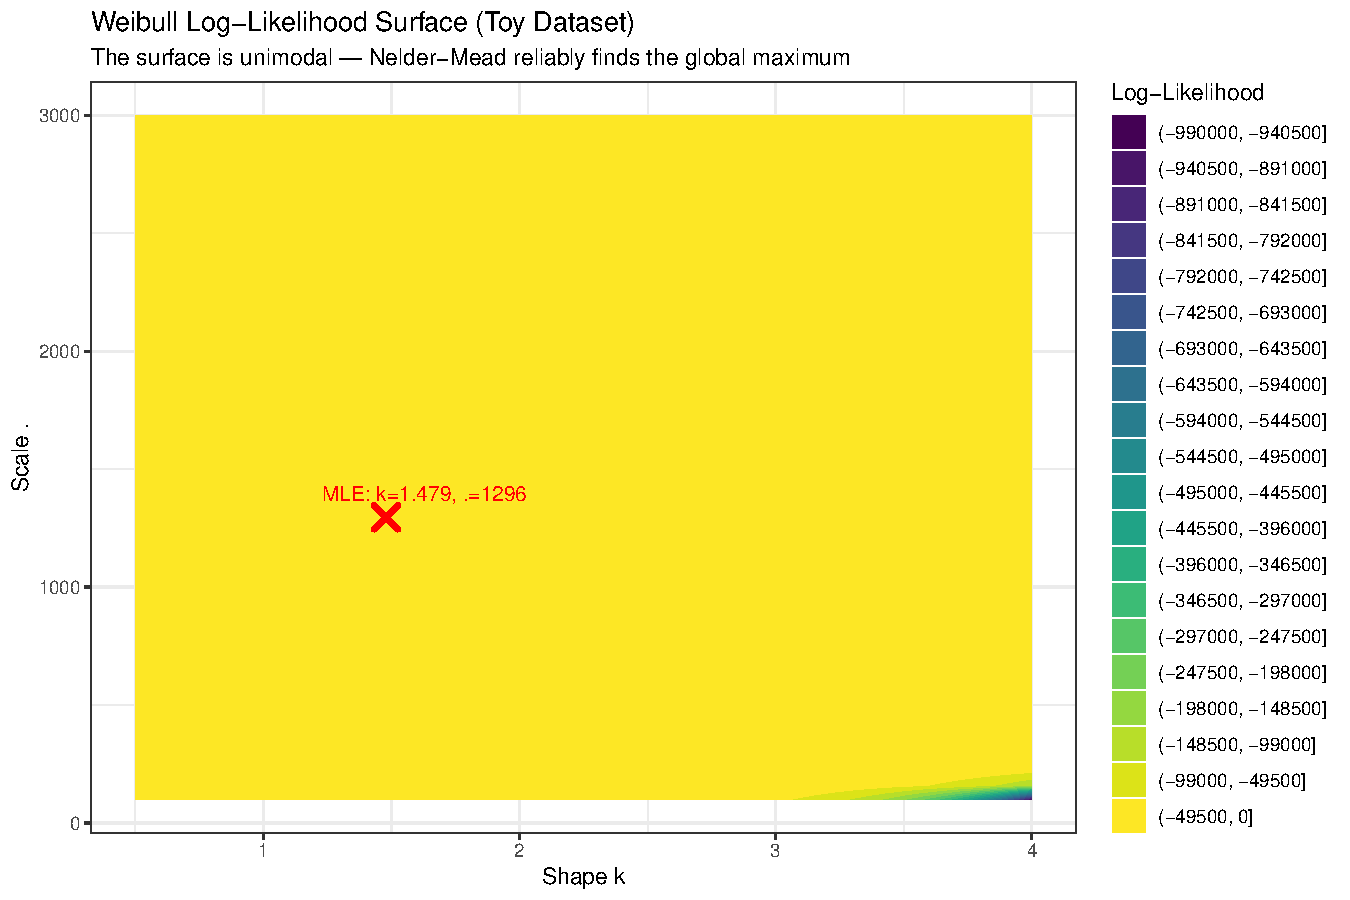
\includegraphics{CODE_EXPLAINED_files/figure-latex/nm-surface-1} 

}

\caption{Weibull log-likelihood surface with MLE optimum}\label{fig:nm-surface}
\end{figure}

\textbf{Nelder-Mead algorithm} (simplex in 2D = triangle of 3 points):

\begin{enumerate}
\def\labelenumi{\arabic{enumi}.}
\tightlist
\item
  Identify best (B), worst (W), middle (M) vertices
\item
  Centroid of non-worst: \(\bar{x} = (B+M)/2\)
\item
  Reflection: \(R = \bar{x} + (\bar{x} - W)\). If better than B → Expand
\item
  If worse than M → Contract: \(C = \bar{x} + 0.5(\bar{x} - W)\)
\item
  If contraction fails → Shrink all toward B
\end{enumerate}

\begin{Shaded}
\begin{Highlighting}[]
\FunctionTok{cat}\NormalTok{(}\StringTok{"MLE results: k ="}\NormalTok{, }\FunctionTok{round}\NormalTok{(k\_mle, }\DecValTok{4}\NormalTok{), }\StringTok{", lambda ="}\NormalTok{, }\FunctionTok{round}\NormalTok{(lam\_mle, }\DecValTok{2}\NormalTok{), }\StringTok{"}\SpecialCharTok{\textbackslash{}n}\StringTok{"}\NormalTok{)}
\end{Highlighting}
\end{Shaded}

\begin{verbatim}
## MLE results: k = 1.4787 , lambda = 1296.02
\end{verbatim}

\begin{Shaded}
\begin{Highlighting}[]
\FunctionTok{cat}\NormalTok{(}\StringTok{"Convergence:"}\NormalTok{, }\FunctionTok{ifelse}\NormalTok{(mle\_res}\SpecialCharTok{$}\NormalTok{convergence }\SpecialCharTok{==} \DecValTok{0}\NormalTok{, }\StringTok{"OK"}\NormalTok{, }\StringTok{"FAILED"}\NormalTok{))}
\end{Highlighting}
\end{Shaded}

\begin{verbatim}
## Convergence: OK
\end{verbatim}

\subsection{2.7A MAP (Bayesian Maximum A
Posteriori)}\label{a-map-bayesian-maximum-a-posteriori}

\subsubsection{2.7.1 Mathematical
Foundation}\label{mathematical-foundation-6}

\textbf{Bayes' theorem}:
\(\pi(k,\lambda | \text{data}) \propto L(\text{data} | k,\lambda) \cdot \pi(k) \cdot \pi(\lambda)\)

\textbf{Flat prior = MLE} (algebraic derivation):
\[\text{If } \pi(k) \propto 1, \pi(\lambda) \propto 1:\]
\[\ln \pi_{\text{post}} = \ln L + \ln(1) + \ln(1) = \ln L\]
\[\text{MAP with flat prior} = \text{MLE exactly.}\]

Our exponential prior: \(\pi(k) \propto e^{-k/\mu_k}\) adds
regularization \(-k/\mu_k\) that penalizes large \(k\).

\begin{Shaded}
\begin{Highlighting}[]
\NormalTok{neg\_logpost }\OtherTok{\textless{}{-}} \ControlFlowTok{function}\NormalTok{(lp) \{}
\NormalTok{  k }\OtherTok{\textless{}{-}} \FunctionTok{exp}\NormalTok{(lp[}\DecValTok{1}\NormalTok{]); lam }\OtherTok{\textless{}{-}} \FunctionTok{exp}\NormalTok{(lp[}\DecValTok{2}\NormalTok{])}
  \ControlFlowTok{if}\NormalTok{ (k }\SpecialCharTok{\textless{}=} \DecValTok{0} \SpecialCharTok{||}\NormalTok{ lam }\SpecialCharTok{\textless{}=} \DecValTok{0}\NormalTok{) }\FunctionTok{return}\NormalTok{(}\FloatTok{1e12}\NormalTok{)}
\NormalTok{  ll }\OtherTok{\textless{}{-}} \FunctionTok{weibull\_loglik}\NormalTok{(k, lam, toy\_t)}
\NormalTok{  log\_prior\_k }\OtherTok{\textless{}{-}} \SpecialCharTok{{-}}\NormalTok{k }\SpecialCharTok{/} \DecValTok{2}          \CommentTok{\# exponential prior, mean=2}
\NormalTok{  log\_prior\_lam }\OtherTok{\textless{}{-}} \SpecialCharTok{{-}}\NormalTok{lam }\SpecialCharTok{/} \FunctionTok{mean}\NormalTok{(toy\_t)}
  \SpecialCharTok{{-}}\NormalTok{(ll }\SpecialCharTok{+}\NormalTok{ log\_prior\_k }\SpecialCharTok{+}\NormalTok{ log\_prior\_lam)}
\NormalTok{\}}

\NormalTok{map\_res }\OtherTok{\textless{}{-}} \FunctionTok{optim}\NormalTok{(}\FunctionTok{c}\NormalTok{(}\FunctionTok{log}\NormalTok{(}\FloatTok{1.5}\NormalTok{), }\FunctionTok{log}\NormalTok{(}\FunctionTok{mean}\NormalTok{(toy\_t))), neg\_logpost, }\AttributeTok{method =} \StringTok{"Nelder{-}Mead"}\NormalTok{)}
\NormalTok{k\_map }\OtherTok{\textless{}{-}} \FunctionTok{exp}\NormalTok{(map\_res}\SpecialCharTok{$}\NormalTok{par[}\DecValTok{1}\NormalTok{]); lam\_map }\OtherTok{\textless{}{-}} \FunctionTok{exp}\NormalTok{(map\_res}\SpecialCharTok{$}\NormalTok{par[}\DecValTok{2}\NormalTok{])}
\FunctionTok{cat}\NormalTok{(}\StringTok{"MAP results: k ="}\NormalTok{, }\FunctionTok{round}\NormalTok{(k\_map, }\DecValTok{4}\NormalTok{), }\StringTok{", lambda ="}\NormalTok{, }\FunctionTok{round}\NormalTok{(lam\_map, }\DecValTok{2}\NormalTok{))}
\end{Highlighting}
\end{Shaded}

\begin{verbatim}
## MAP results: k = 1.381 , lambda = 1207.62
\end{verbatim}

\subsection{2.7B MCMC (Full Bayesian ---
Extension)}\label{b-mcmc-full-bayesian-extension}

\textbf{NOTE}: This method is an EXTENSION beyond the core course
documents.

\begin{itemize}
\tightlist
\item
  \textbf{MAP} gives one point (the posterior mode). False precision
  with small samples.
\item
  \textbf{MCMC} gives the full posterior distribution. Wide credible
  intervals are honest, not a weakness.
\end{itemize}

\begin{Shaded}
\begin{Highlighting}[]
\CommentTok{\# MCMC Implementation via brms/Stan}
\NormalTok{fit }\OtherTok{\textless{}{-}} \FunctionTok{brm}\NormalTok{(}
\NormalTok{  lifetime\_days }\SpecialCharTok{|}\NormalTok{ \FunctionTok{cens}\NormalTok{(}\DecValTok{1} \SpecialCharTok{{-}}\NormalTok{ failed) }\SpecialCharTok{\textasciitilde{}} \DecValTok{1}\NormalTok{,}
  \AttributeTok{data    =}\NormalTok{ drive\_data,}
  \AttributeTok{family  =} \FunctionTok{weibull}\NormalTok{(),}
  \AttributeTok{prior   =} \FunctionTok{c}\NormalTok{(}
    \FunctionTok{prior}\NormalTok{(}\FunctionTok{exponential}\NormalTok{(}\FloatTok{0.5}\NormalTok{), }\AttributeTok{class =}\NormalTok{ shape),            }\CommentTok{\# k prior}
    \FunctionTok{prior}\NormalTok{(}\FunctionTok{normal}\NormalTok{(}\DecValTok{0}\NormalTok{, }\DecValTok{10}\NormalTok{), }\AttributeTok{class =}\NormalTok{ Intercept)            }\CommentTok{\# log(lambda) prior}
\NormalTok{  ),}
  \AttributeTok{chains  =} \DecValTok{4}\NormalTok{, }\AttributeTok{iter =} \DecValTok{2000}\NormalTok{, }\AttributeTok{cores =} \DecValTok{4}
\NormalTok{)}

\CommentTok{\# Extracting k and lambda from posterior}
\NormalTok{draws }\OtherTok{\textless{}{-}} \FunctionTok{as\_draws\_df}\NormalTok{(fit)}
\NormalTok{k\_draws }\OtherTok{\textless{}{-}}\NormalTok{ draws}\SpecialCharTok{$}\NormalTok{shape}
\NormalTok{lam\_draws }\OtherTok{\textless{}{-}} \FunctionTok{exp}\NormalTok{(draws}\SpecialCharTok{$}\NormalTok{b\_Intercept) }\SpecialCharTok{/} \FunctionTok{gamma}\NormalTok{(}\DecValTok{1} \SpecialCharTok{+} \DecValTok{1}\SpecialCharTok{/}\NormalTok{k\_draws)}

\FunctionTok{cat}\NormalTok{(}\StringTok{"MCMC Result: k ="}\NormalTok{, }\FunctionTok{median}\NormalTok{(k\_draws), }\StringTok{"| lambda ="}\NormalTok{, }\FunctionTok{median}\NormalTok{(lam\_draws))}
\end{Highlighting}
\end{Shaded}

MCMC uses Hamiltonian Monte Carlo (HMC/NUTS via Stan), an efficient
modern sampling algorithm. Key diagnostics:

\begin{itemize}
\tightlist
\item
  \textbf{Rhat \textless{} 1.01}: within-chain vs between-chain variance
  must agree
\item
  \textbf{ESS \textgreater{} 400}: effective independent samples after
  accounting for autocorrelation
\item
  \textbf{pp\_check}: simulated data from posterior should match
  observed data
\end{itemize}

\subsection{2.8 Percentile}\label{percentile}

\begin{Shaded}
\begin{Highlighting}[]
\NormalTok{p1 }\OtherTok{\textless{}{-}} \FloatTok{0.16}\NormalTok{; p2 }\OtherTok{\textless{}{-}} \FloatTok{0.84}
\NormalTok{t1 }\OtherTok{\textless{}{-}} \FunctionTok{quantile}\NormalTok{(toy\_t, p1, }\AttributeTok{names =} \ConstantTok{FALSE}\NormalTok{)}
\NormalTok{t2 }\OtherTok{\textless{}{-}} \FunctionTok{quantile}\NormalTok{(toy\_t, p2, }\AttributeTok{names =} \ConstantTok{FALSE}\NormalTok{)}

\NormalTok{k\_pct }\OtherTok{\textless{}{-}}\NormalTok{ (}\FunctionTok{log}\NormalTok{(}\SpecialCharTok{{-}}\FunctionTok{log}\NormalTok{(}\DecValTok{1}\SpecialCharTok{{-}}\NormalTok{p2)) }\SpecialCharTok{{-}} \FunctionTok{log}\NormalTok{(}\SpecialCharTok{{-}}\FunctionTok{log}\NormalTok{(}\DecValTok{1}\SpecialCharTok{{-}}\NormalTok{p1))) }\SpecialCharTok{/}\NormalTok{ (}\FunctionTok{log}\NormalTok{(t2) }\SpecialCharTok{{-}} \FunctionTok{log}\NormalTok{(t1))}
\NormalTok{lam\_pct }\OtherTok{\textless{}{-}}\NormalTok{ t1 }\SpecialCharTok{/}\NormalTok{ (}\SpecialCharTok{{-}}\FunctionTok{log}\NormalTok{(}\DecValTok{1}\SpecialCharTok{{-}}\NormalTok{p1))}\SpecialCharTok{\^{}}\NormalTok{(}\DecValTok{1}\SpecialCharTok{/}\NormalTok{k\_pct)}

\FunctionTok{cat}\NormalTok{(}\StringTok{"t1 (p=0.16) ="}\NormalTok{, }\FunctionTok{round}\NormalTok{(t1, }\DecValTok{1}\NormalTok{), }\StringTok{"| t2 (p=0.84) ="}\NormalTok{, }\FunctionTok{round}\NormalTok{(t2, }\DecValTok{1}\NormalTok{), }\StringTok{"}\SpecialCharTok{\textbackslash{}n}\StringTok{"}\NormalTok{)}
\end{Highlighting}
\end{Shaded}

\begin{verbatim}
## t1 (p=0.16) = 445.6 | t2 (p=0.84) = 1902
\end{verbatim}

\begin{Shaded}
\begin{Highlighting}[]
\FunctionTok{cat}\NormalTok{(}\StringTok{"Percentile results: k ="}\NormalTok{, }\FunctionTok{round}\NormalTok{(k\_pct, }\DecValTok{4}\NormalTok{), }\StringTok{", lambda ="}\NormalTok{, }\FunctionTok{round}\NormalTok{(lam\_pct, }\DecValTok{2}\NormalTok{))}
\end{Highlighting}
\end{Shaded}

\begin{verbatim}
## Percentile results: k = 1.621 , lambda = 1308.95
\end{verbatim}

Uses only 2 of 10 points. The remaining 8 contribute nothing. Expected
to perform worst.

\subsection{Summary: All Methods on Toy
Dataset}\label{summary-all-methods-on-toy-dataset}

\begin{Shaded}
\begin{Highlighting}[]
\NormalTok{toy\_results }\OtherTok{\textless{}{-}} \FunctionTok{tibble}\NormalTok{(}
  \AttributeTok{Method =} \FunctionTok{c}\NormalTok{(}\StringTok{"OLS"}\NormalTok{, }\StringTok{"WLS"}\NormalTok{, }\StringTok{"MOM"}\NormalTok{, }\StringTok{"L{-}Moments"}\NormalTok{, }\StringTok{"EPF"}\NormalTok{, }\StringTok{"MLE"}\NormalTok{, }\StringTok{"MAP"}\NormalTok{, }\StringTok{"Percentile"}\NormalTok{),}
  \AttributeTok{k =} \FunctionTok{c}\NormalTok{(k\_ols, k\_wls, k\_mom, k\_closed, k\_epf\_exact, k\_mle, k\_map, k\_pct),}
  \AttributeTok{lambda =} \FunctionTok{c}\NormalTok{(lam\_ols, lam\_wls, lam\_mom, lam\_lmom, lam\_epf, lam\_mle, lam\_map, lam\_pct)}
\NormalTok{) }\SpecialCharTok{\%\textgreater{}\%}
  \FunctionTok{mutate}\NormalTok{(}\FunctionTok{across}\NormalTok{(}\FunctionTok{c}\NormalTok{(k, lambda), }\SpecialCharTok{\textasciitilde{}}\FunctionTok{round}\NormalTok{(., }\DecValTok{4}\NormalTok{)))}

\NormalTok{toy\_results }\SpecialCharTok{\%\textgreater{}\%}
  \FunctionTok{kable}\NormalTok{(}\AttributeTok{caption =} \StringTok{"Toy Dataset — All Methods Comparison"}\NormalTok{,}
        \AttributeTok{booktabs =} \ConstantTok{TRUE}\NormalTok{) }\SpecialCharTok{\%\textgreater{}\%}
  \FunctionTok{kable\_styling}\NormalTok{(}\AttributeTok{latex\_options =} \FunctionTok{c}\NormalTok{(}\StringTok{"striped"}\NormalTok{, }\StringTok{"hold\_position"}\NormalTok{))}
\end{Highlighting}
\end{Shaded}

\begin{longtable}[t]{lrr}
\caption{\label{tab:toy-summary}Toy Dataset — All Methods Comparison}\\
\toprule
Method & k & lambda\\
\midrule
\cellcolor{gray!10}{OLS} & \cellcolor{gray!10}{1.1881} & \cellcolor{gray!10}{1345.69}\\
WLS & 1.2852 & 1335.70\\
\cellcolor{gray!10}{MOM} & \cellcolor{gray!10}{1.4369} & \cellcolor{gray!10}{1293.12}\\
L-Moments & 1.2901 & 1269.16\\
\cellcolor{gray!10}{EPF} & \cellcolor{gray!10}{1.5718} & \cellcolor{gray!10}{1307.20}\\
\addlinespace
MLE & 1.4787 & 1296.02\\
\cellcolor{gray!10}{MAP} & \cellcolor{gray!10}{1.3810} & \cellcolor{gray!10}{1207.62}\\
Percentile & 1.6210 & 1308.95\\
\bottomrule
\end{longtable}

\newpage

\section{Chapter 3 --- Goodness of Fit}\label{chapter-3-goodness-of-fit}

\subsection{3.1 KS (Kolmogorov-Smirnov)}\label{ks-kolmogorov-smirnov}

\(KS = \max_i |F_{\text{emp}}(t_i) - F_{\text{fit}}(t_i)|\) --- the
L\(_\infty\) norm.

\textbf{CAVEAT 1}: When parameters are estimated from the same data, the
KS test becomes conservative. Do not compare against standard KS
critical values.

\textbf{CAVEAT 2}: Standard KS does not handle right-censored data.
Computed over failure times only --- approximate.

\begin{Shaded}
\begin{Highlighting}[]
\CommentTok{\# Step 1: Get fitted CDF at sorted failure times}
\NormalTok{F\_fit }\OtherTok{\textless{}{-}} \FunctionTok{pweibull}\NormalTok{(t\_sorted, }\AttributeTok{shape =}\NormalTok{ k\_mle, }\AttributeTok{scale =}\NormalTok{ lam\_mle)}

\CommentTok{\# Step 2: Maximum absolute difference}
\NormalTok{KS }\OtherTok{\textless{}{-}} \FunctionTok{max}\NormalTok{(}\FunctionTok{abs}\NormalTok{(F\_i }\SpecialCharTok{{-}}\NormalTok{ F\_fit))}
\FunctionTok{cat}\NormalTok{(}\StringTok{"KS Metric ="}\NormalTok{, }\FunctionTok{round}\NormalTok{(KS, }\DecValTok{5}\NormalTok{))}
\end{Highlighting}
\end{Shaded}

\begin{verbatim}
## KS Metric = 0.05445
\end{verbatim}

\subsection{3.2 RMSE vs MAE}\label{rmse-vs-mae}

\begin{itemize}
\tightlist
\item
  \textbf{RMSE} =
  \(\sqrt{\frac{1}{n}\sum(F_{\text{emp}} - F_{\text{fit}})^2}\) ---
  L\(_2\) norm, squares large errors
\item
  \textbf{MAE} = \(\frac{1}{n}\sum|F_{\text{emp}} - F_{\text{fit}}|\)
  --- L\(_1\) norm, equal weight
\end{itemize}

Always \(\text{MAE} \leq \text{RMSE}\). If
\(\text{RMSE} \gg \text{MAE}\): one or few badly fitted points.

\begin{Shaded}
\begin{Highlighting}[]
\NormalTok{RMSE }\OtherTok{\textless{}{-}} \FunctionTok{sqrt}\NormalTok{(}\FunctionTok{mean}\NormalTok{((F\_i }\SpecialCharTok{{-}}\NormalTok{ F\_fit)}\SpecialCharTok{\^{}}\DecValTok{2}\NormalTok{))}
\NormalTok{MAE  }\OtherTok{\textless{}{-}} \FunctionTok{mean}\NormalTok{(}\FunctionTok{abs}\NormalTok{(F\_i }\SpecialCharTok{{-}}\NormalTok{ F\_fit))}

\FunctionTok{cat}\NormalTok{(}\StringTok{"RMSE ="}\NormalTok{, }\FunctionTok{round}\NormalTok{(RMSE, }\DecValTok{5}\NormalTok{), }\StringTok{"| MAE ="}\NormalTok{, }\FunctionTok{round}\NormalTok{(MAE, }\DecValTok{5}\NormalTok{))}
\end{Highlighting}
\end{Shaded}

\begin{verbatim}
## RMSE = 0.03522 | MAE = 0.03011
\end{verbatim}

\subsection{3.3 Anderson-Darling}\label{anderson-darling}

\[A^2 = -n - \frac{1}{n}\sum_{i=1}^n (2i-1)[\ln(z_i) + \ln(1-z_{n+1-i})]\]

Weight table: \(w(u) = 1/[u(1-u)]\)

{\def\LTcaptype{none} % do not increment counter
\begin{longtable}[]{@{}lll@{}}
\toprule\noalign{}
\(u\) & Weight & Multiplier vs baseline \\
\midrule\noalign{}
\endhead
\bottomrule\noalign{}
\endlastfoot
0.50 & 4.0 & 1.0× \\
0.10 & 11.1 & 2.8× \\
0.05 & 21.1 & 5.3× \\
0.02 & 51.0 & 12.8× \\
\end{longtable}
}

\begin{Shaded}
\begin{Highlighting}[]
\CommentTok{\# Implementation: Standardize residuals by expected variance}
\NormalTok{z     }\OtherTok{\textless{}{-}}\NormalTok{ F\_fit}
\NormalTok{z\_rev }\OtherTok{\textless{}{-}} \FunctionTok{rev}\NormalTok{(z)}
\NormalTok{AD }\OtherTok{\textless{}{-}} \SpecialCharTok{{-}}\NormalTok{n }\SpecialCharTok{{-}} \NormalTok{(}\DecValTok{1}\SpecialCharTok{/}\NormalTok{n) }\SpecialCharTok{*} \FunctionTok{sum}\NormalTok{((}\DecValTok{2}\SpecialCharTok{*}\NormalTok{i }\SpecialCharTok{{-}} \DecValTok{1}\NormalTok{) }\SpecialCharTok{*}\NormalTok{ (}\FunctionTok{log}\NormalTok{(z) }\SpecialCharTok{+} \FunctionTok{log}\NormalTok{(}\DecValTok{1} \SpecialCharTok{{-}}\NormalTok{ z\_rev)))}

\FunctionTok{cat}\NormalTok{(}\StringTok{"Anderson{-}Darling (A²) ="}\NormalTok{, }\FunctionTok{round}\NormalTok{(AD, }\DecValTok{4}\NormalTok{))}
\end{Highlighting}
\end{Shaded}

\begin{verbatim}
## Anderson-Darling (A²) = 0.2312
\end{verbatim}

\subsection{3.4 AIC and AICc}\label{aic-and-aicc}

\(\text{AIC} = -2\ell + 2p\), corrected:
\(\text{AICc} = \text{AIC} + \frac{2p(p+1)}{n-p-1}\)

\textbf{CAVEAT}: Theoretically valid for MLE only. For non-MLE methods,
used as comparative convenience.

\(\Delta\)AIC interpretation: 0--2 (both supported), 2--6 (moderate),
6--10 (strong), \textgreater10 (very strong).

\begin{Shaded}
\begin{Highlighting}[]
\CommentTok{\# Recompute log-likelihood including CENSORED items}
\NormalTok{censored\_loglik }\OtherTok{\textless{}{-}} \ControlFlowTok{function}\NormalTok{(t, event, k, lam) \{}
\NormalTok{  t\_ratio }\OtherTok{\textless{}{-}}\NormalTok{ t }\SpecialCharTok{/}\NormalTok{ lam}
\NormalTok{  ll\_fail }\OtherTok{\textless{}{-}} \FunctionTok{sum}\NormalTok{(event }\SpecialCharTok{*}\NormalTok{ (}\FunctionTok{log}\NormalTok{(k) }\SpecialCharTok{{-}} \FunctionTok{log}\NormalTok{(lam) }\SpecialCharTok{+} \NormalTok{(k}\SpecialCharTok{{-}}\DecValTok{1}\NormalTok{)}\SpecialCharTok{*}\FunctionTok{log}\NormalTok{(t\_ratio) }\SpecialCharTok{{-}}\NormalTok{ t\_ratio}\SpecialCharTok{\^{}}\NormalTok{k))}
\NormalTok{  ll\_cens }\OtherTok{\textless{}{-}} \FunctionTok{sum}\NormalTok{((}\DecValTok{1}\SpecialCharTok{{-}}\NormalTok{event) }\SpecialCharTok{*}\NormalTok{ (}\SpecialCharTok{{-}}\NormalTok{t\_ratio}\SpecialCharTok{\^{}}\NormalTok{k))}
  \FunctionTok{return}\NormalTok{(ll\_fail }\SpecialCharTok{+}\NormalTok{ ll\_cens)}
\NormalTok{\}}

\NormalTok{ll }\OtherTok{\textless{}{-}} \FunctionTok{censored\_loglik}\NormalTok{(toy\_t, }\FunctionTok{rep}\NormalTok{(}\DecValTok{1}\NormalTok{, n), k\_mle, lam\_mle)}
\NormalTok{AIC }\OtherTok{\textless{}{-}} \SpecialCharTok{{-}}\DecValTok{2}\SpecialCharTok{*}\NormalTok{ll }\SpecialCharTok{+} \DecValTok{2}\SpecialCharTok{*}\DecValTok{2}
\FunctionTok{cat}\NormalTok{(}\StringTok{"AIC ="}\NormalTok{, }\FunctionTok{round}\NormalTok{(AIC, }\DecValTok{2}\NormalTok{))}
\end{Highlighting}
\end{Shaded}

\begin{verbatim}
## AIC = 162.45
\end{verbatim}

\subsection{3.5 MRL Error}\label{mrl-error}

\[\text{MRL}_{\%} = \frac{|\hat{\mu}_{\text{fit}} - \bar{t}_f|}{\bar{t}_f} \times 100\]

\textbf{CAVEAT}: \(\bar{t}_f\) uses only failures. Under heavy
censoring, it is downward-biased.

\begin{Shaded}
\begin{Highlighting}[]
\NormalTok{MTTF\_pred }\OtherTok{\textless{}{-}}\NormalTok{ lam\_mle }\SpecialCharTok{*} \FunctionTok{gamma}\NormalTok{(}\DecValTok{1} \SpecialCharTok{+} \DecValTok{1}\SpecialCharTok{/}\NormalTok{k\_mle)}
\NormalTok{MTTF\_obs  }\OtherTok{\textless{}{-}} \FunctionTok{mean}\NormalTok{(toy\_t)}
\NormalTok{MRL\_err   }\OtherTok{\textless{}{-}} \FunctionTok{abs}\NormalTok{(MTTF\_pred }\SpecialCharTok{{-}}\NormalTok{ MTTF\_obs) }\SpecialCharTok{/}\NormalTok{ MTTF\_obs }\SpecialCharTok{*} \DecValTok{100}
\FunctionTok{cat}\NormalTok{(}\StringTok{"MRL Error ="}\NormalTok{, }\FunctionTok{round}\NormalTok{(MRL\_err, }\DecValTok{2}\NormalTok{), }\StringTok{"\%"}\NormalTok{)}
\end{Highlighting}
\end{Shaded}

\subsection{3.6 Composite Rank}\label{composite-rank}

\(R_{\text{composite}} = \frac{r_{\text{RMSE}} + r_{\text{AD}} + r_{\text{AIC}}}{3}\)
--- Borda count.

Why these three: RMSE (global body), AD (tail-sensitive), AIC
(likelihood-based with censoring). Rank normalization prevents AIC from
dominating.

\begin{Shaded}
\begin{Highlighting}[]
\CommentTok{\# Composite Rank Calculation}
\NormalTok{model\_gof }\OtherTok{\textless{}{-}}\NormalTok{ model\_gof }\SpecialCharTok{\%\textgreater{}\%}
  \FunctionTok{mutate}\NormalTok{(}
    \AttributeTok{rank\_RMSE =} \FunctionTok{rank}\NormalTok{(RMSE),}
    \AttributeTok{rank\_AD   =} \FunctionTok{rank}\NormalTok{(AD),}
    \AttributeTok{rank\_AIC  =} \FunctionTok{rank}\NormalTok{(AIC),}
    \AttributeTok{Composite =}\NormalTok{ (rank\_RMSE }\SpecialCharTok{+}\NormalTok{ rank\_AD }\SpecialCharTok{+}\NormalTok{ rank\_AIC) }\SpecialCharTok{/} \DecValTok{3}
\NormalTok{  )}
\end{Highlighting}
\end{Shaded}

\newpage

\section{Chapter 4 --- Reading the
Plots}\label{chapter-4-reading-the-plots}

\subsection{Weibull Probability Plot}\label{weibull-probability-plot}

\begin{itemize}
\tightlist
\item
  \textbf{Straight line} = data follows Weibull distribution
\item
  \textbf{Curvature upward right} = heavier tail than Weibull
  (lognormal?)
\item
  \textbf{Curvature downward} = lighter tail
\item
  \textbf{Slope} = \(k\) (shape parameter)
\item
  \textbf{Diverging lines} = methods disagree on \(k\) --- check with
  GoF metrics
\end{itemize}

\subsection{Survival Function (Kaplan-Meier Benchmark)}\label{survival-function-kaplan-meier-benchmark}

The \textbf{Kaplan-Meier (KM)} curve serves as the non-parametric ``ground truth'' benchmark for survival probabilities.
\begin{itemize}
\tightlist
\item
  \textbf{Flat curve near 1.0}: Due to the heavily right-censored nature of the data (most drives survive the window), the true empirical reliability curve remains very close to 1.0. 
\item
  \textbf{Accounting for Censoring}: The KM estimator mathematically accounts for drives that survive beyond the observation window, unlike raw failure rank plotting.
\item
  \textbf{Method Comparison}: Often reveals when WLS estimators overfit to early infant mortality (falling below the KM curve) while MLE and MCMC remain securely aligned with the true population survival rate.
\end{itemize}

\subsection{Hazard Function}\label{hazard-function}

\begin{itemize}
\tightlist
\item
  \(k < 1\): decreasing hazard --- \textbf{infant mortality} (burn-in
  helps)
\item
  \(k = 1\): constant hazard --- \textbf{random failures} (memoryless,
  replacement scheduling useless)
\item
  \(k > 1\): increasing hazard --- \textbf{wear-out} (preventive
  replacement beneficial)
\item
  \(k \approx 3.5\): approximates normal distribution shape
\end{itemize}

\subsection{GoF Heatmap}\label{gof-heatmap}

\begin{itemize}
\tightlist
\item
  Consistently green row = robustly best method
\item
  Wins RMSE but loses AD = body fits but tail misfit
\item
  WLS green where MLE red = model is slightly misspecified
\end{itemize}

\subsection{Parameter Plot}\label{parameter-plot}

\begin{itemize}
\tightlist
\item
  Wide MCMC error bars = data cannot pin down parameter precisely
\item
  MLE outside MCMC CI = likelihood surface may be irregular
\end{itemize}

\newpage

\section{Chapter 5 --- Decision Logic}\label{chapter-5-decision-logic}

\begin{Shaded}
\begin{Highlighting}[]
\CommentTok{\#  START: Compute censoring fraction}
\CommentTok{\#    ↓}
\CommentTok{\#  censoring \textgreater{} 0\%? → Eliminate: Percentile, MOM, EPF}
\CommentTok{\#    ↓}
\CommentTok{\#  censoring \textgreater{} \textasciitilde{}5\%? → Also eliminate: L{-}Moments}
\CommentTok{\#    ↓  }
\CommentTok{\#  censoring \textgreater{} \textasciitilde{}20\%? → Also eliminate: OLS, WLS}
\CommentTok{\#    ↓}
\CommentTok{\#  Surviving methods retained}
\CommentTok{\#    ↓}
\CommentTok{\#  Prior knowledge? YES → MAP (7A) or MCMC (7B)}
\CommentTok{\#                   NO  → MLE}
\CommentTok{\#    ↓}
\CommentTok{\#  Compute composite GoF for surviving methods}
\CommentTok{\#    ↓}
\CommentTok{\#  Select best method → REPORT}
\end{Highlighting}
\end{Shaded}

\textbf{WLS can outrank MLE}: If the true distribution is only
approximately Weibull, MLE's commitment to the exact functional form is
a liability. WLS fits the empirical CDF more loosely. Always run GoF ---
never assume MLE wins.

\newpage

\section{Session Info}\label{session-info}

\begin{Shaded}
\begin{Highlighting}[]
\FunctionTok{sessionInfo}\NormalTok{()}
\end{Highlighting}
\end{Shaded}

\begin{verbatim}
## R version 4.5.2 (2025-10-31 ucrt)
## Platform: x86_64-w64-mingw32/x64
## Running under: Windows 11 x64 (build 26200)
## 
## Matrix products: default
##   LAPACK version 3.12.1
## 
## locale:
## [1] LC_COLLATE=French_Tunisia.utf8  LC_CTYPE=French_Tunisia.utf8   
## [3] LC_MONETARY=French_Tunisia.utf8 LC_NUMERIC=C                   
## [5] LC_TIME=French_Tunisia.utf8    
## 
## time zone: Africa/Tunis
## tzcode source: internal
## 
## attached base packages:
## [1] stats     graphics  grDevices utils     datasets  methods   base     
## 
## other attached packages:
##  [1] kableExtra_1.4.0 knitr_1.51       here_1.0.2       lubridate_1.9.5 
##  [5] forcats_1.0.1    stringr_1.6.0    dplyr_1.2.1      purrr_1.2.2     
##  [9] readr_2.2.0      tidyr_1.3.2      tibble_3.3.1     ggplot2_4.0.2   
## [13] tidyverse_2.0.0 
## 
## loaded via a namespace (and not attached):
##  [1] gtable_0.3.6       compiler_4.5.2     tidyselect_1.2.1   xml2_1.5.2        
##  [5] textshaping_1.0.5  systemfonts_1.3.2  scales_1.4.0       yaml_2.3.12       
##  [9] fastmap_1.2.0      R6_2.6.1           labeling_0.4.3     generics_0.1.4    
## [13] isoband_0.3.0      rprojroot_2.1.1    svglite_2.2.2      pillar_1.11.1     
## [17] RColorBrewer_1.1-3 tzdb_0.5.0         rlang_1.2.0        stringi_1.8.7     
## [21] xfun_0.57          S7_0.2.1           viridisLite_0.4.3  timechange_0.4.0  
## [25] cli_3.6.6          withr_3.0.2        magrittr_2.0.5     digest_0.6.39     
## [29] grid_4.5.2         rstudioapi_0.18.0  hms_1.1.4          lifecycle_1.0.5   
## [33] vctrs_0.7.3        evaluate_1.0.5     glue_1.8.1         farver_2.1.2      
## [37] rmarkdown_2.31     tools_4.5.2        pkgconfig_2.0.3    htmltools_0.5.9
\end{verbatim}

\end{document}
